\chapter{Consumer Group Autoscaler} \label{chap:consumer_group_autoscaler}

\section{Problem Formulation}

As shown in figure \ref{fig:problem_context}, the data pipeline consists of
extracting data from Kafka topics and inserting it into a data lake to be
further treated in the remaining ETL processes.  The work developed throughout
this thesis, is based on optimizing the pipeline from Kafka into BigQuery, by
providing a dynamic solution that makes use of Kafka's parallelism without
disregarding the cost of the number of instances deployed. 

The aim is to achieve a deterministic approach as for the number of consumers
required working in parallel, so as to guarantee that the rate of production
into a topic is not higher than the rate of consumption, which would lead to
messages being accumulated in a topic making the lag increase between the last
message inserted and the last message read by the consumer group.

A Kafka topic is subdivided into several partitions, distributed within the
several brokers of the Kafka cluster. When sending a message into a topic, if a
key is provided, then the message will consistently end up in the same
partition, whereas if none is provided, then the message is inserted in a
round-robin fashion in one of the partitions of the same topic. Messages going
into a topic may also have different sizes ($bytes$), and for these reasons, the
write speed ($bytes/s$) to the several partitions in a topic is not guaranteed
to be the same. 

The following model, also assumes that the maximum consumption rate of a single
consumer is constant, and if there is enough data to be consumed, this is the
speed the consumer functions at when working "full throttle". This is
elaborated in section \ref{result:bin capacity} based on several tests performed
to determine this value for a consumer. 

Based on the previous information, the model for this pipeline is considered to
fit the constraints for the SBSBPP, where the consumer is the bin that has as
capacity its maximum consumption rate, and the weights are the partitions and
their respective write speeds. The problem then is to find the minimum amount of
consumers where to fit all the partitions so as to make sure that the sum of the
write speeds of the partitions assigned to a single consumer does not exceed its
maximum capacity. 

For a single iteration, the optimal solution finds the arrangement between the
partitions and the consumers that minimizes the amount of instances, but this
solution is not static, as the write speeds of the partitions changes with time.
As such, there is a second factor to take into consideration which is the
partition reassignment. 

When a partition is reassigned, because 2 consumers from the same group cannot
be consuming from the same partition at a time, when assigning a partition to
another consumer, the one it is currently assigned to has to stop consuming in
order to allow the new consumer to start. Due to this process, there is some
downtime where data is not being consumed from a partition.

For this reason, making use of an optimal algorithm that also minimizes
partition redistribution, is not feasible as it would not run within the
necessary time requirements due to the NP hard nature of the problem.  To
determine the arrangement of partitions and consumers, this work is based on the
studied approximation algorithms which have already been mentioned in the
literature review. As is clear, there is no approximation algorithm which
considers item redistribution. The reason for this may lay on the fact that the
context where this problem lies is not very common, and there is no mention of a
stateful assignment where each item is already assigned a bin prior to executing
the algorithm.

Due to the dynamic nature of the problem the items change in size depending on
the measurement performed at time instant $t$. Consequently, constraint
\ref{opt:c1} is remodeled to take the time instant $t$ at which the algorithm is
to be executed into account.
\begin{alignat}{3}
\label{BPP model}
    &\min       
        &&\sum_{i \in B} y_i 
            && \\
    &\text{subject to} \quad
        && \sum_{j \in L} \hat w_j(t) \cdot x_{ij} \leq y_i. \quad      
            && \forall \; i \in B \\
    &   && \sum_{i \in B} x_{ij} = 1, \quad                             
            && \forall \; j \in L \\
    &   && y_i \in \{0, 1\}                                             
            && \forall \; i \in B \\
    &   && x_{ij} \in \{0,1\}                                           
            && \forall \; i \in B, j \in L
\end{alignat}

Time instant $t$ represents an instant at which a measurement was performed
of the items' sizes, leading to a new computation of the bin packing assignment.
Since an assignment represents a consumer reading data from the partition, an
item can also be reassigned to another consumer (bin) adding a new variation to the
traditional BPP. 

\begin{figure}[htb!] \centering
    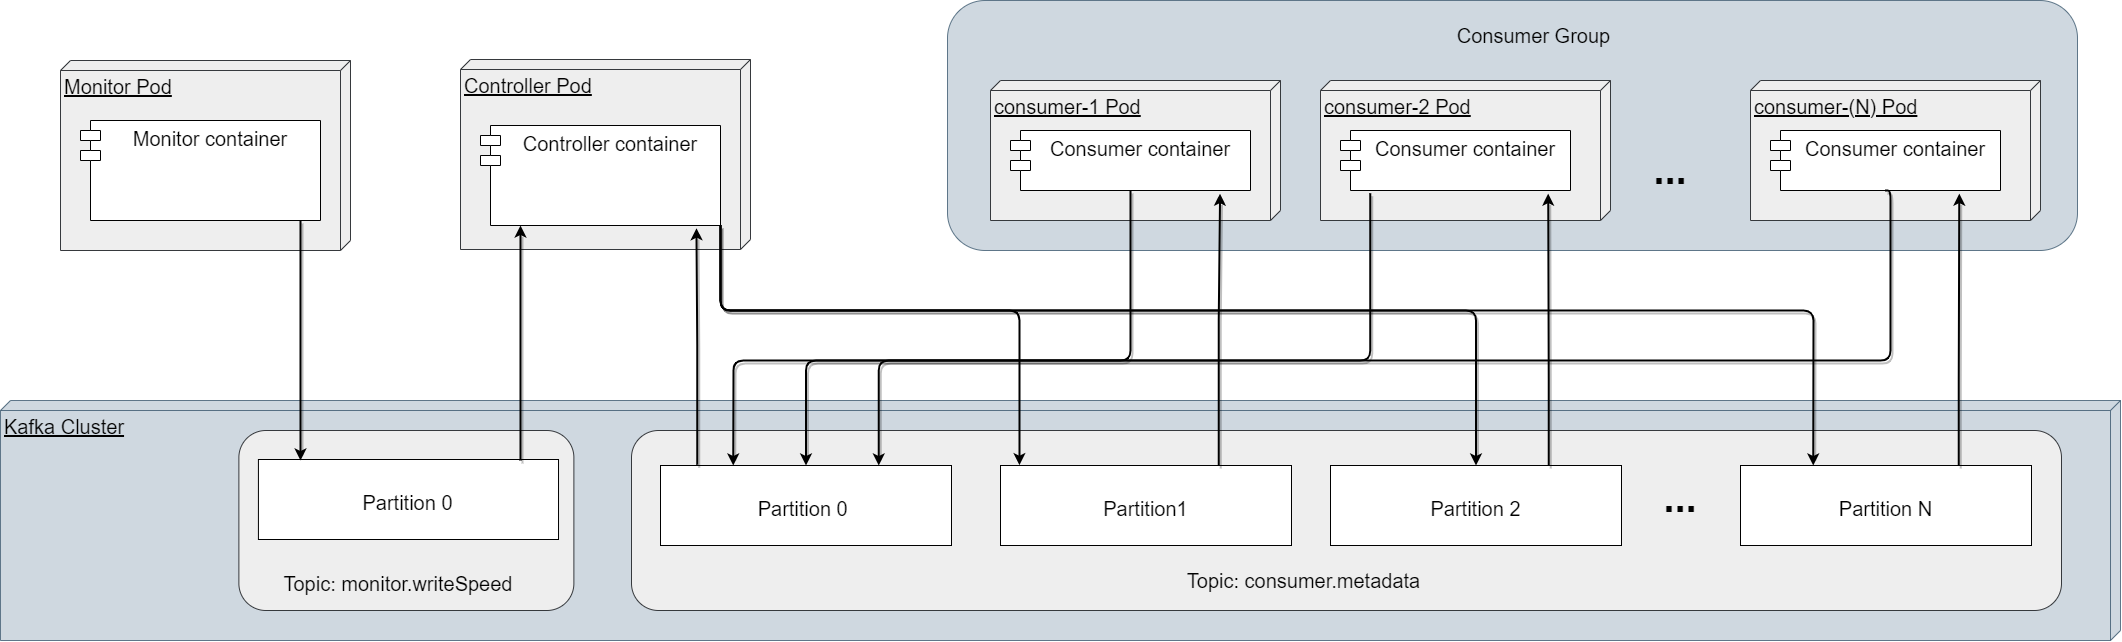
\includegraphics[width=\textwidth]{images/controller/System Design.png}
    \caption{System architecture deployment diagram} 
    \label{fig:system_architecture}
\end{figure}

As presented in figure \ref{fig:system_architecture}, there are three components
that interact with one another in order to model the problem as a BPP, and to
provide a fully dynamic pipeline capable of autoscaliing based on the current
load of data being produced to the partitions of interest.

The monitor process is responsible for measuring the write speed of each
partition the group is interested in consuming data from, which is equivalent to
specifying the size of the items of the BPP.  This information is then delivered
to the controller, which is responsible for managing a consumer group (creating
and deleting consumer instances), and mapping each partition to a consumer. The
consumers are then informed of their tasks and read the data from the partitions
that were assigned to them by the controller.

\begin{comment}
    The Data-Engineering (DE) team at HUUB is responsible for making a pipeline that
    inserts data from several data sources into a data lake so it can then be
    transformed and loaded into a single source of truth data warehouse. 

    HUUB's current architecture makes use of event sourcing to announce events that
    change the system's state within a microservice. Prior to this architecture, it
    was common to fetch the information from several different databases which were
    of interest for this department, periodically and in batches, which lead to
    tight coupling between the work performed by the different teams at the company.

    Based on reporting and real-time data needs, with regards to the extraction
    process, if there is new data that has to be consumed from a service that isn't
    currently being consumed, Kafka and event sourcing allow this addition to be as
    simple as subscribing the DE consumer to the topic of interest.
\end{comment}

\section{Monitor} \label{component:Monitor}

\IncMargin{1em} 
\begin{algorithm}[h]
    \SetKwData{Left}{left}
    \SetKwData{This}{this}
    \SetKwData{Up}{up}
    \SetKwFunction{Union}{Union}
    \SetKwFunction{FindCompress}{FindCompress}
    \SetKwInOut{Input}{input} 
    \Input{ 
        admin - Kafka admin client to communicate with cluster, \\ 
        producer - Kafka producer client, \\ 
        topics - list of topic identifiers from which the monitor is to
        determine the speed of their partitions 
    } 
    \BlankLine

    measurementQueue $\gets$ Queue<Measurement>()\; 
    \While{true}{ 
        measurement $\gets$ new Measurement()\; 
        measurement.partitionSizes $\gets$ admin.getLogDirs(topics)\; 
        measurement.timestamp $\gets$ currentTime()\;
        measurementQueue.add(measurement)\; 
        \If{(measurementQueue.first.timestamp - measurement.last.timestamp) > 30s}{ 
            sizeDiff $\gets$ measurement.last.partitionSizes - measurement.first.partitionSizes\;
            timeDiff $\gets$ measurement.last.timestamp - measurement.first.timestamp\;
            measurementSpeed $\gets$ sizeDiff / timeDiff\;
            producer.producer("monitor.writeSpeed", measurementSpeed)
            \While{(currentTime() - measurementQueue.first.timestamp) > 30s}{
                measurementQueue.pop()\; 
            } 
        } 
    } 
    \caption{Monitor process pseudo-code.}
\label{algo:monitor} \end{algorithm}\DecMargin{1em}

To solve the BPP, initially the controller requires as input the write speed of
each partition the consumer group is interested in consuming data from. The
monitor process is responsible for providing this information.

If enabled, Kafka exposes metrics to external java processes through Java
Management Extensions (JMX). Prometheus can then be used as a wrapper to these
metrics as it creates a unified model to query the data, and it also registers
the data as a timeseries, allowing for a historic view of any parameter, as well
as creating more elaborate metrics over the exposed cluster metrics. At the time
of writing this thesis and to the best of my knowledge, there is no available
metric that provides a partition's write speed.  For this reason, this section
aims to explain the process that is responsible for monitoring the write speed
of the partitions of interest.

Kafka provides an Admin client, which can be used to administer the cluster, and
also query information about it. This client/class exposes a method
\lstinline[language=Python]{describeLogDirs()} which queries the cluster for the
amount of bytes each TopicPartition has. A TopicPartition is a string-integer
pair, which identifies any partition (integer) within a topic (string). 

Since the consumer only consumes from the partition leader, if the
\lstinline[language=Python]{replication-factor > 1}, then several partitions are
excluded from the result of the previous method call, since this process is only
interested in the partitions that belong to one of the topics of interest, and
which are leaders.

Each time the partition size is queried by the admin client, a timestamp is
appended to the measurement, and it is inserted to the back of the queue. Any
query that is older than $30s$, which is guaranteed to be in the front of the
queue, is removed. To obtain the write speed of a single partition, the last
element of the queue and the first (representing the latest and the earliest
measurement of the partition size within the last $30s$) are used to compute the
ratio between the difference in bytes and the difference in time ($bytes/s$).
This is also the average write speed over the last 30 seconds.

Every topic has the parameters \lstinline[language=Python]{retention.ms} and
\lstinline[language=Python]{retention.bytes}, which determine how long a record
remains in a partition before being deleted, or how many bytes a partition
retains before removing old records. When a record is deleted, the partition
size reduces as it no longer reserves space for the removed record. For this
process to have an accurate write speed, it is important to set both of these
parameter to \lstinline[language=Python]{-1}, which means that the record is
never deleted from the partition. Ideally, the admin client would be able query
for the historic size of a partition, but since this information could not be
retrieved, this approach was what was implemented.

After computing the write speed for all the partitions of interest, the message
has to be communicated to the controller/orchestrator that runs the algorithm to
assign the partitions to the consumers. To benefit from an asynchronous
approach, this monitor process communicates with the controller/orchestrator
process via a kafka topic named
\lstinline[language=Python]{monitor.writeSpeed}, as shown in figure
\ref{fig:system_architecture}. The data to be inserted
is the write speed of the partitions of interest, which is then consumed by the
controller/orchestrator to be used as input for the algorithm's execution.

Two testing scenarios were developed to illustrate the measured partition write
speeds by this method when a controlled producer is sending records at a
predefined rate. The payload inserted into the partition is always 123 bytes.

The first scenario has the producer send the message at 3 different rates for
approximately 35 seconds each. As can be seen in figure \ref{fig:monitor_step},
the monitor increases the measured write speed rate slower than the actual speed
as measured by the producer, since the monitor takes into consideration the
first and last measurement made in the last 30 seconds, whereas the producer
simply measures the produce rate since the last time it inserted a record into
the partition. It takes the monitor 30 seconds to converge to the actual
production speed where it then settles until the produce rate increases again.

\begin{figure}[htb!] 
    \centering
    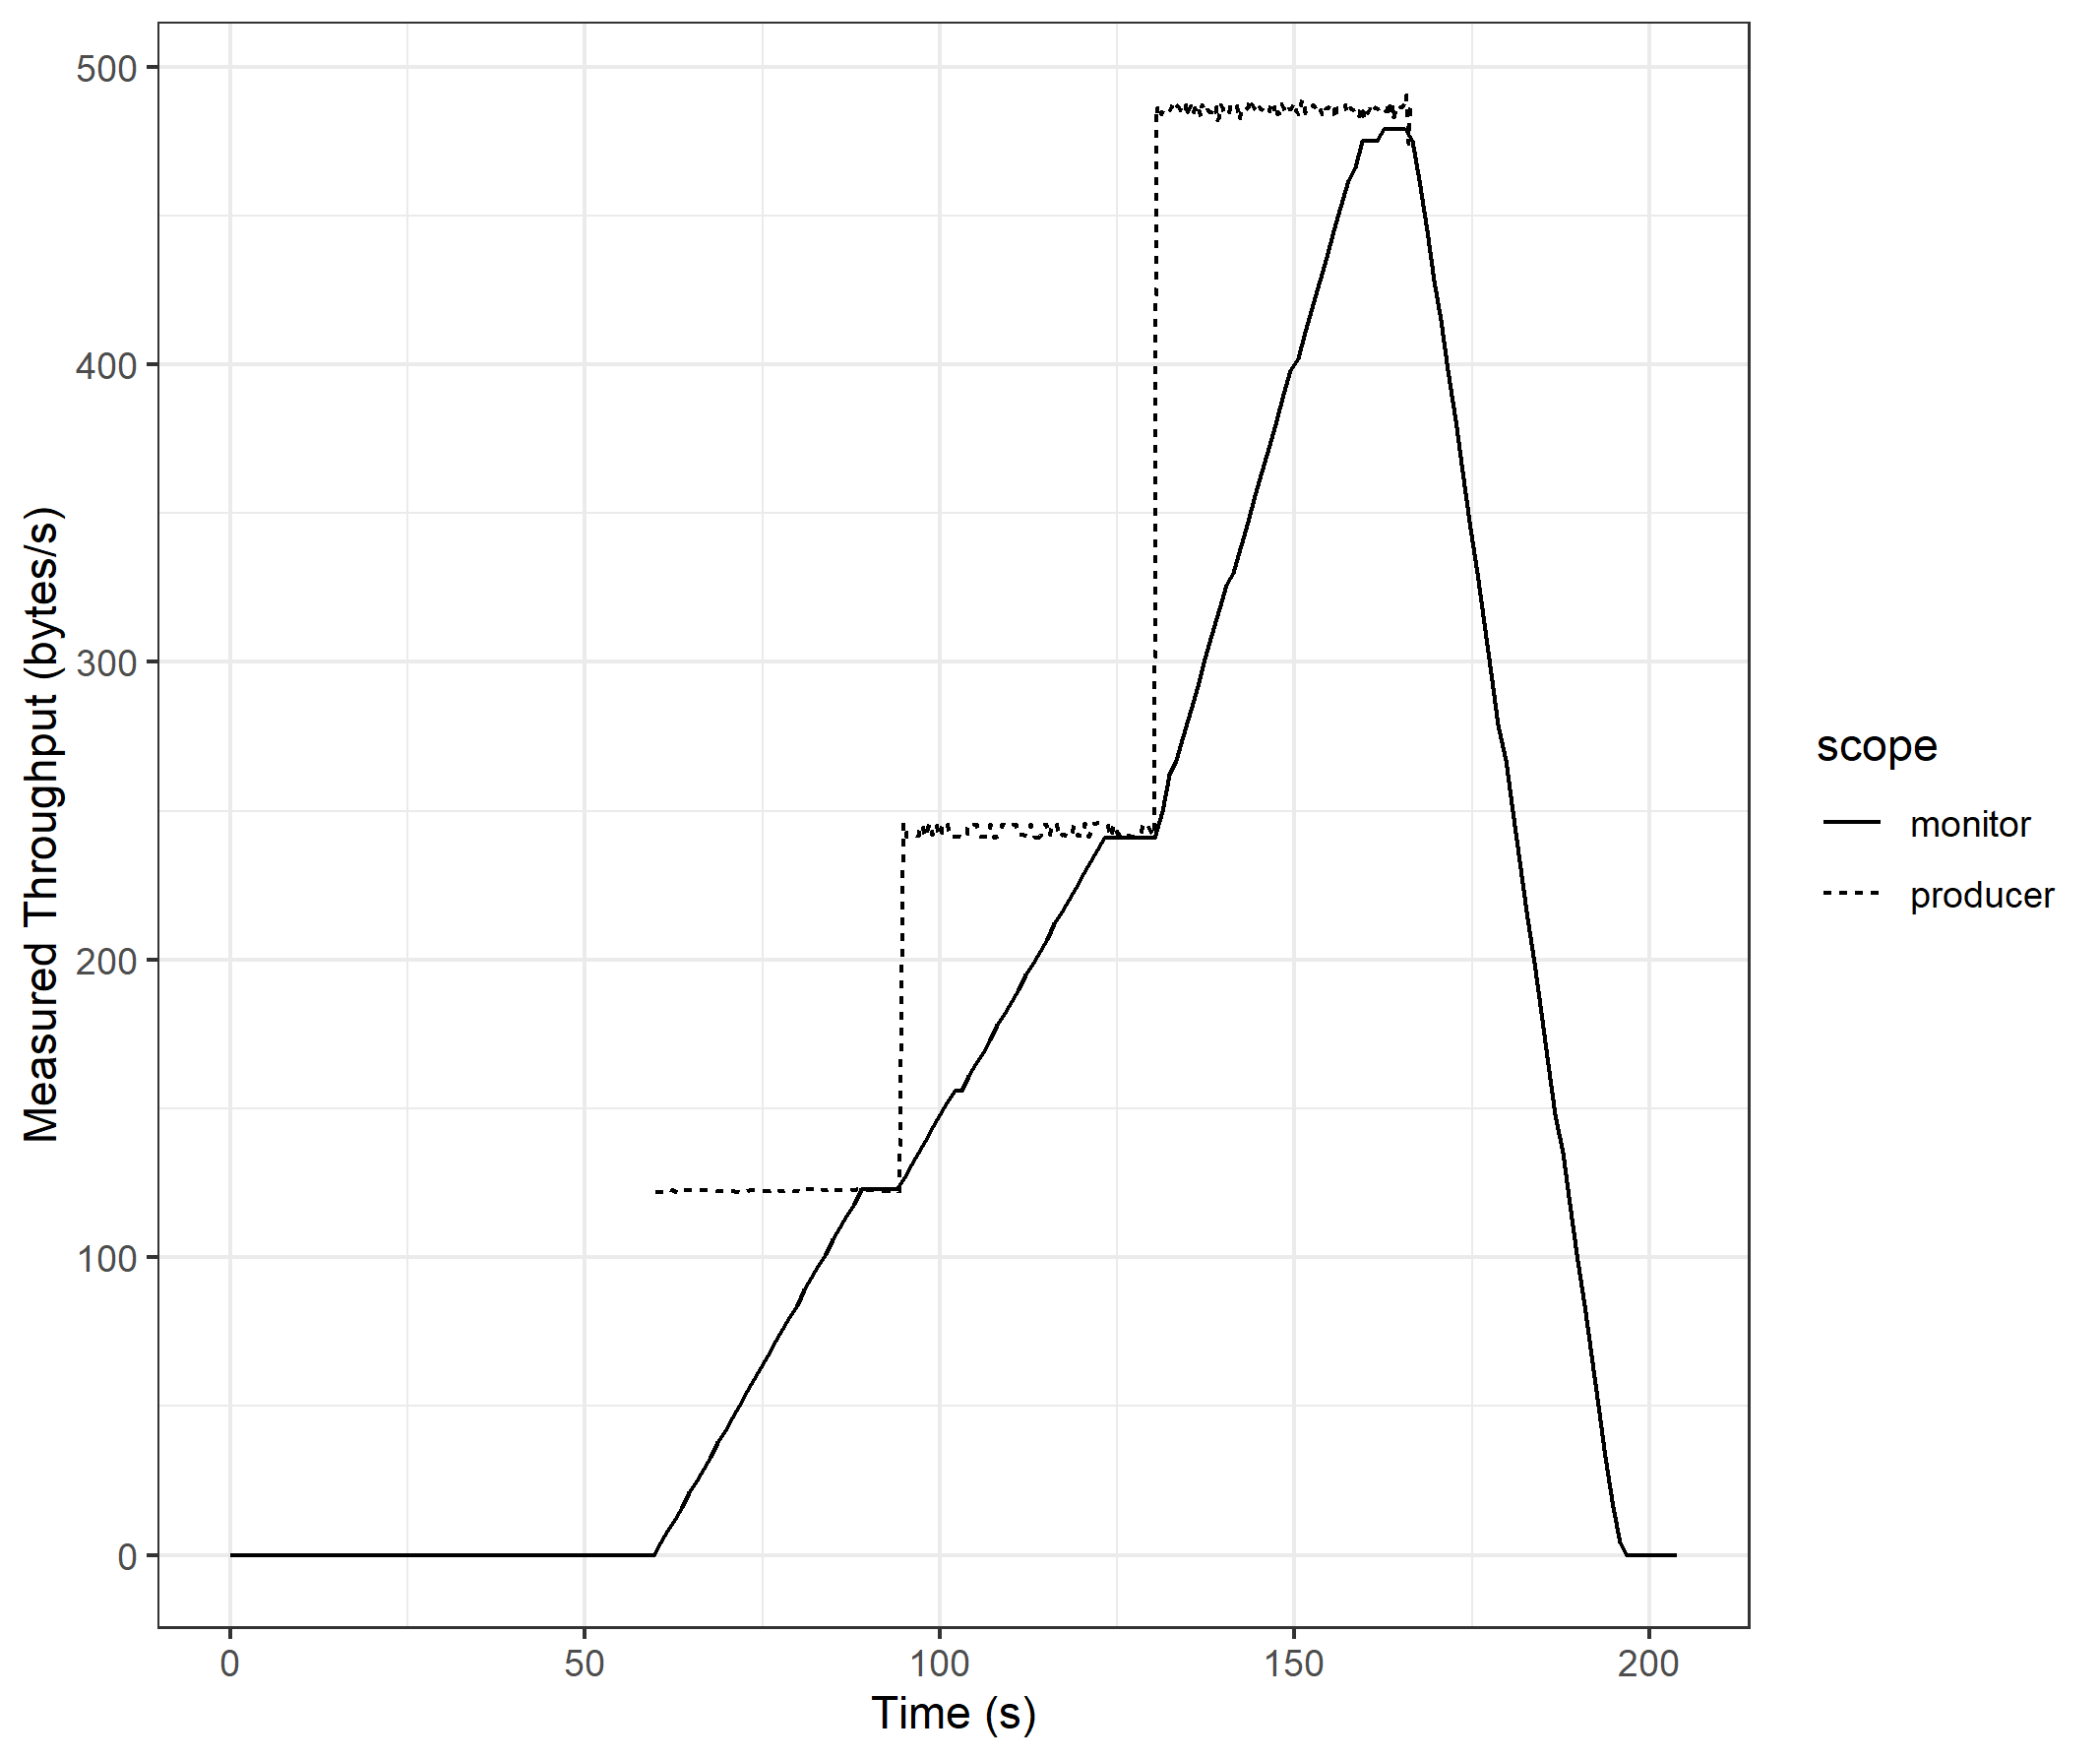
\includegraphics[width=0.7\textwidth]{images/monitor/step.png}
    \caption{Monitor step response to three different controlled write speeds.}
    \label{fig:monitor_step} 
\end{figure}

The second scenario has the producer wait a randomized time interval (between
$[0.01, 2]$ seconds), before sending the message to the partition. Since the
monitor takes into consideration the last 30 seconds from its latest
measurement, it is not affected by the noisy write speed as measured by the
producer. Within these testing conditions, due to the wait time being modeled as
a uniform random variable, the monitor process should stabilize at approximately
the speed computed using the number of bytes produced and the expected wait
time, which in this case is 123 bytes and approximately 1 second respectively.
This is in fact the case as can be seen in figure \ref{fig:monitor_random},
since the write speed stabilizes around $123 bytes/s$. Subfigure (b) from
\ref{fig:monitor_random} presents a statistical description of the producer's
measured write speed, that better illustrates the noise reduction in the
monitor's measurement due to the average.
\begin{figure}[!htb] 
    \centering
    \subfigure[]{
        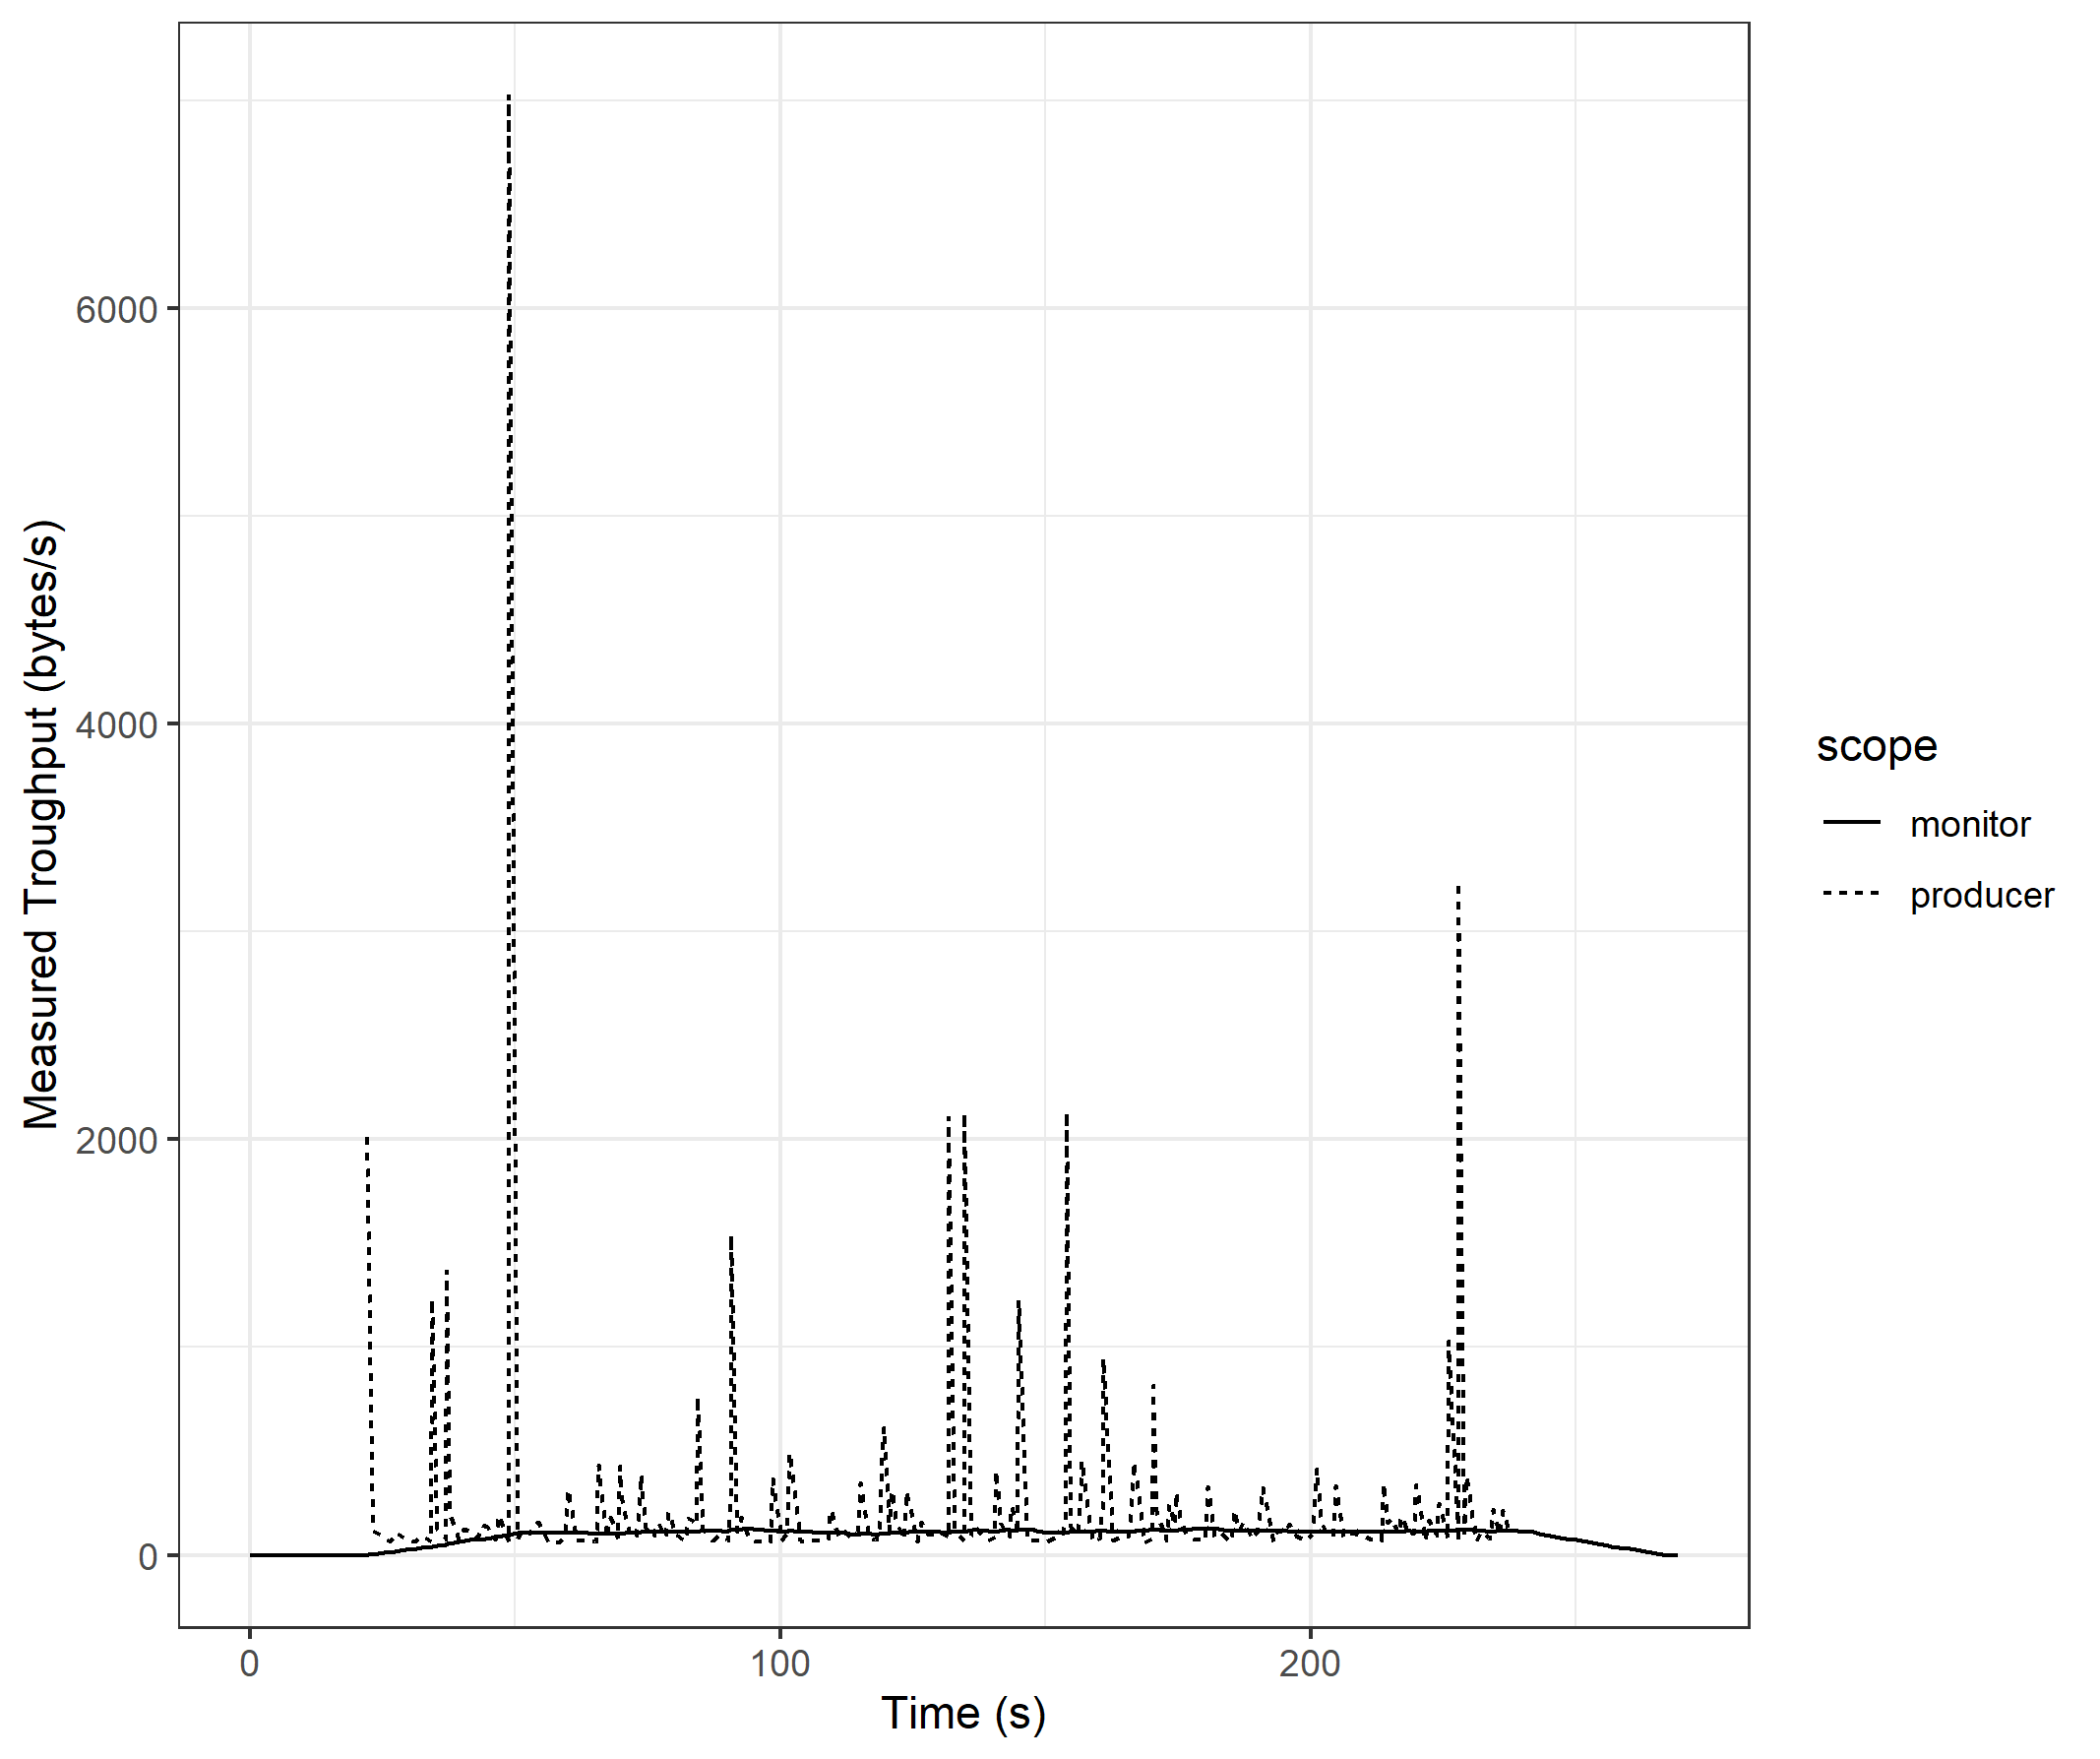
\includegraphics[width=0.4\textwidth]{images/monitor/random_without_boxplot.png}
    }
    \subfigure[]{
        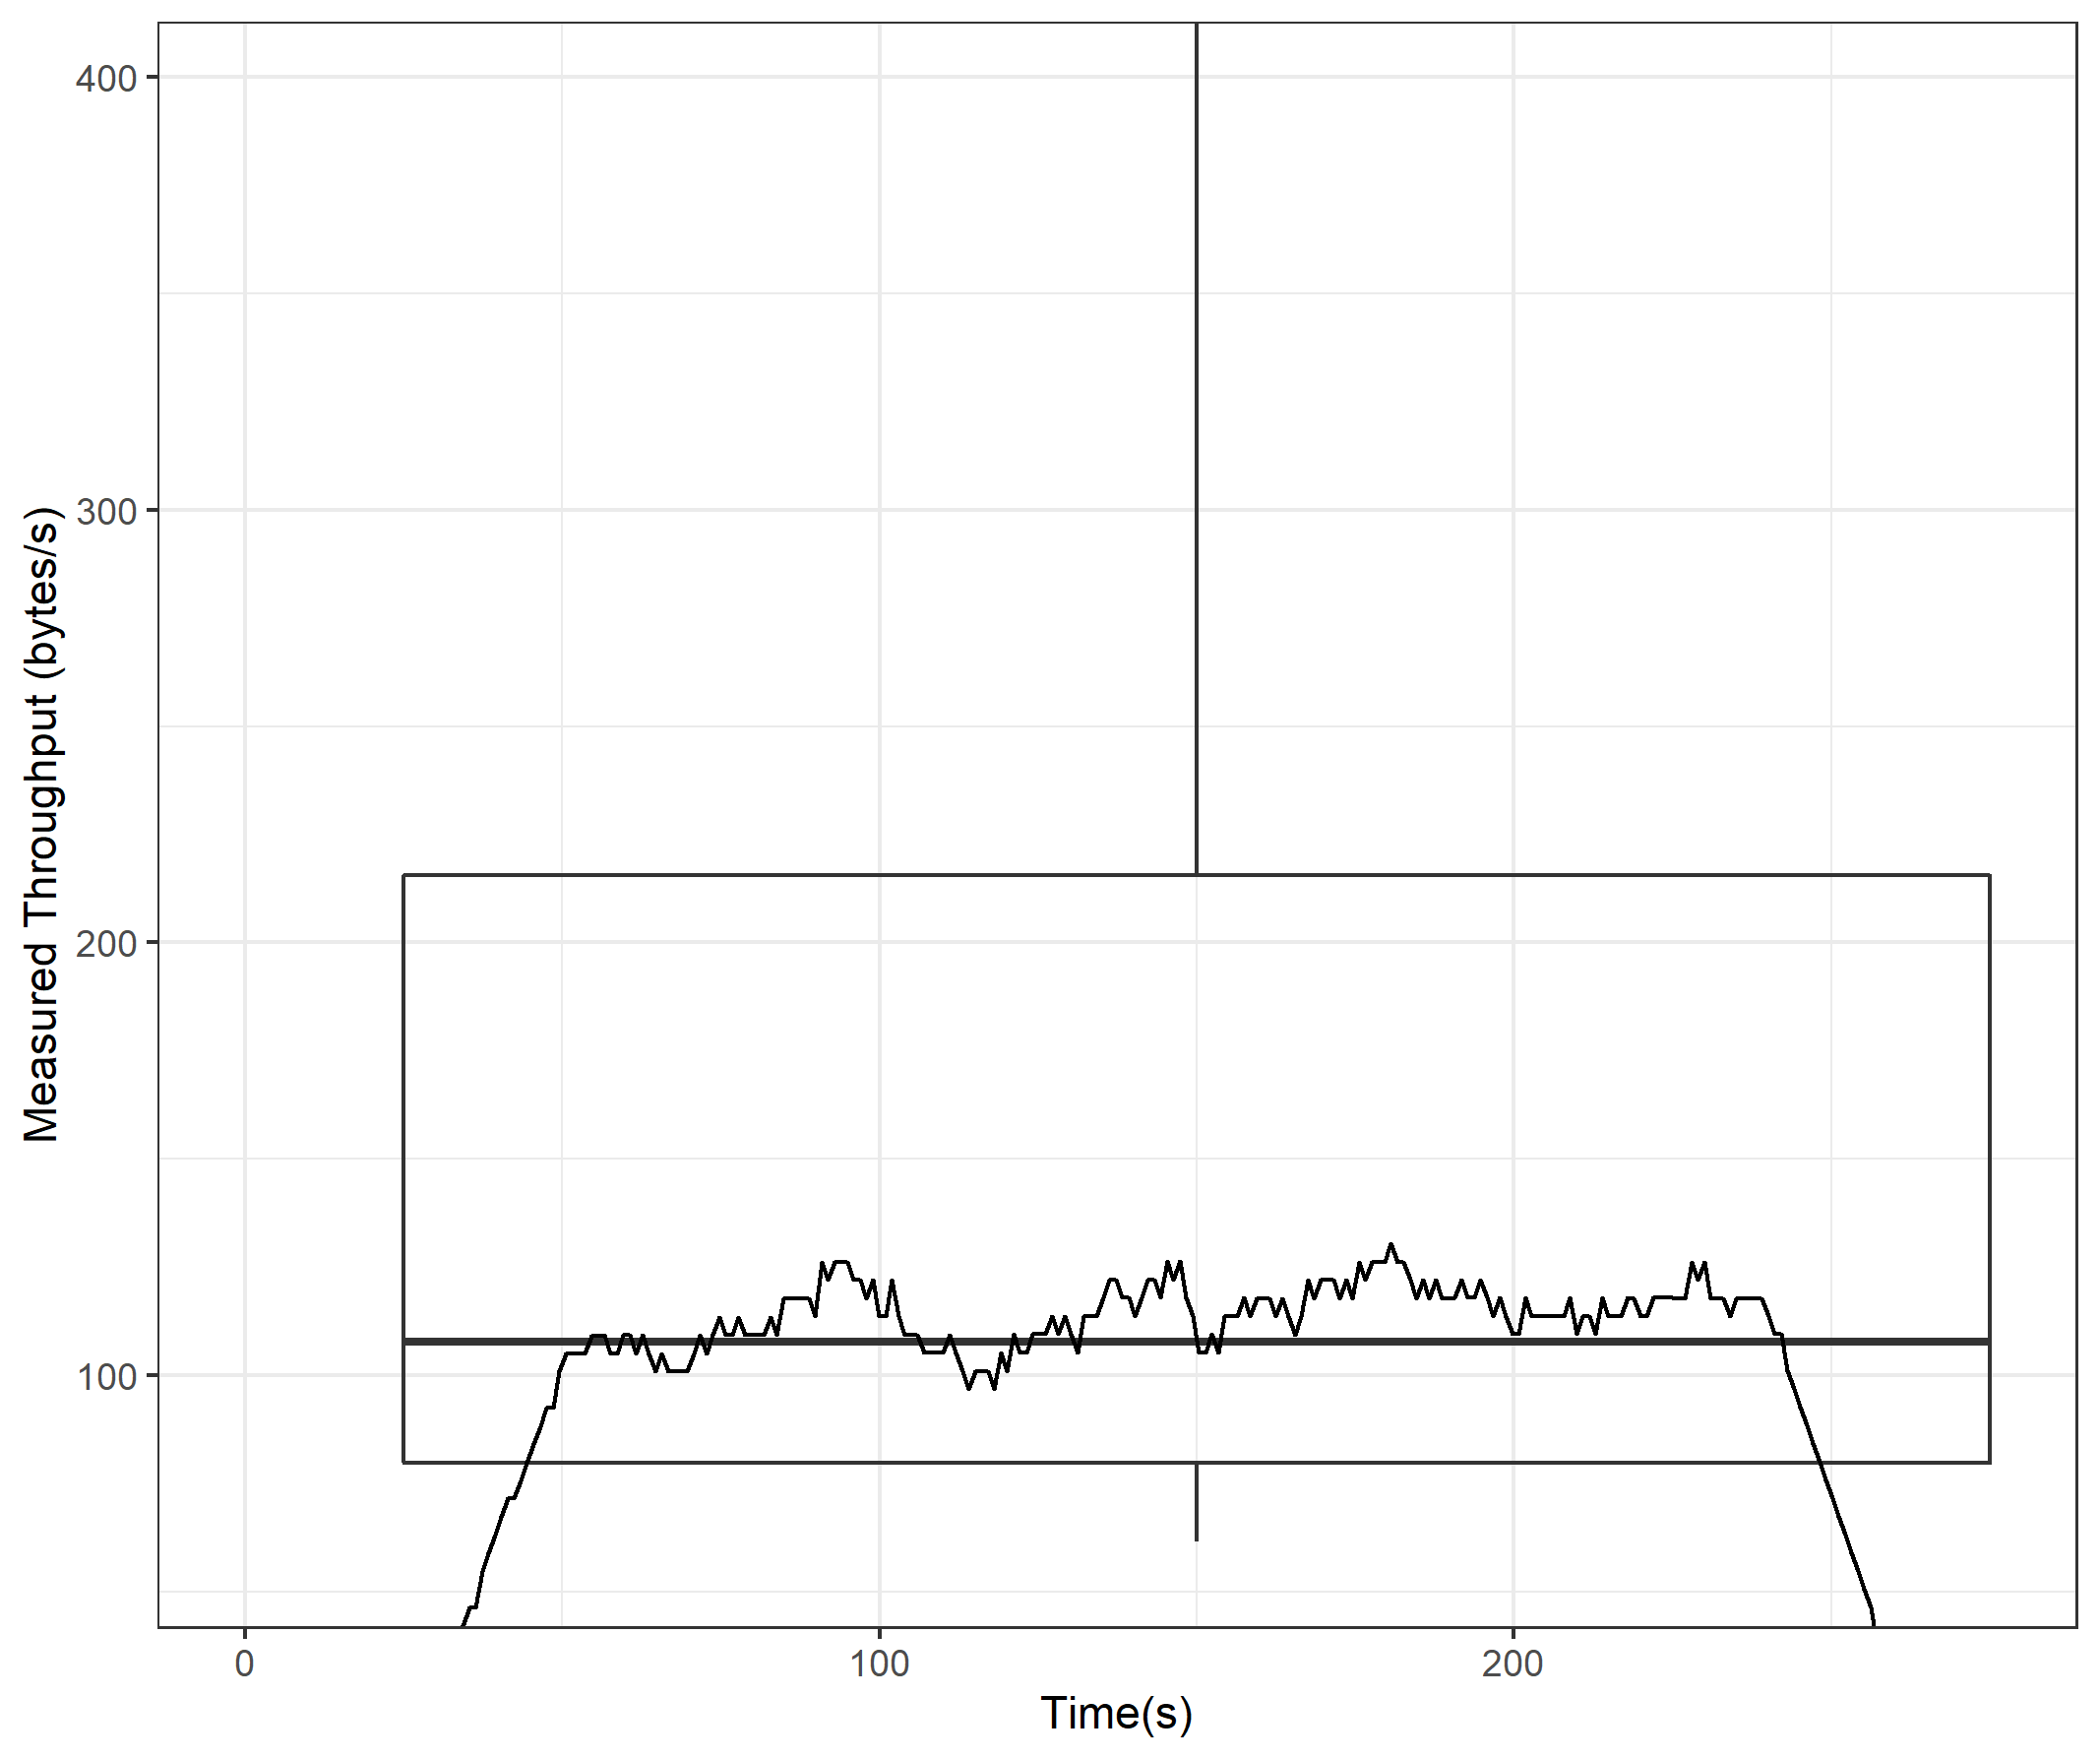
\includegraphics[width=0.4\textwidth]{images/monitor/random_with_boxplot.png}
    }
    \caption{
        (a) Monitor response to a producer waiting uniformely between [0.01,2]s
        every time it produces a record, along with the producer's speed
        measured between each production instance.
        (b) Monitor response to a producer waiting uniformely between [0.01,2]s
        every time it produces a record, with the producer's measured speed
        statistically summarized using a boxplot.
    } 
    \label{fig:monitor_random} 
\end{figure}


\section{Consumer} \label{component:consumer}

The Consumer goes through four important phases within its process, to
approximate its consumption rate to a constant value when being challenged to
work at its peak performance. These phases repeat cyclically until the consumer
is terminated by an external termination signal. 

\subsection{Phase 1: Gathering Records}

The first phase is where data is gathered before being sent to the data
warehouse. The consumer is configured with two important parameters,
\lstinline[language=Python]{BATCH_BYTES} and
\lstinline[language=Python]{WAIT_TIME_SECS}, which indicate respectively, the
amount of bytes the consumer waits to gather in a single iteration, and the
amount of time it is allowed to wait to gather the information.

\subsection{Phase 2: Processing} \label{consumer:phase2}

\IncMargin{1em} 
\begin{algorithm}[h]
    \SetKwData{Left}{left}
    \SetKwData{This}{this}
    \SetKwData{Up}{up}
    \SetKwFunction{Union}{Union}
    \SetKwFunction{FindCompress}{FindCompress}
    \SetKwInOut{Input}{input}
    \SetKwInOut{Output}{output} 
    \Input{\\ 
        messages - List of Kafka messages, \\ 
        mapTopicsTable - Map that indicates which table a message from a topic
            is inserted into 
    } 
    \Output{List<BatchList>} 
    \BlankLine

    mapTableBatchlist $\leftarrow$ new Map[String, BatchList]()\; 
    \For{msg in messages}{ 
        table $\leftarrow$ mapTopicTable.get(msg.topic())\; 
        batchList $\leftarrow$ mapTableBatchlist.get(table)\; 
        \If{(batchList == None)} {
            mapTableBatchlist[table] $\leftarrow$ new BatchList()\; 
            batchList $\leftarrow$ mapTableBatchlist.get(table)\; 
        } 
        batchList.add(msg)\; 
    }
    \KwRet{mapTableBatchlist.values()} 
\caption{Consumer Phase 2 algorithm}
\label{algo:phase_2} 
\end{algorithm} 
\DecMargin{1em}

The second phase is where the data gathered in the previous phase is prepared to
be sent into bigquery. Each record fetched from a Kafka topic, represents a new
row in a bigquery table. 

To insert data into bigquery, Google's Python Bigquery Client is used. Each post
request made with this client, has a batch of rows sent to a single table, and
it is also limited to no more than $10Mbytes$ per request.

Since the gathered records originate from multiple topics, each row has to be
batched with data of its kind, which are rows that are intended to be sent to
the same bigquery table.  A single instance of a Batch, a data structure created
to agglomerate rows intended for the same bigquery table, holds all the rows
which will be sent in a single post request through Google's python bigquery
client API. Due to the imposed limit of a post request, a Batch has a payload
limit of $5 Mbytes$.  A BatchList, is another data structure created to group
instances of type Batch that refer to the same table.

To process the data, a map stores the link between a table's id and the
BatchList instance assigned to it. When analyzing a message, its topic metadata
indicates which table it is directed to, which in turn points to the BatchList
it must be added to.  When adding a message to a BatchList instance, this class
controls to which Batch it is assigned, based on the size of the row, and the
size of the last created Batch within this data structure.

\subsection{Phase 3: Sending Data into Bigquery}

This is the final stage of the consumer's insert cycle. There is a list of
BatchList instances, each having to be sent to a single bigquery table. To
optimize the insert cycle, this phase is done asynchronously with respect to all
the batches within the list of BatchLists contained in the map specified in
algorithm \ref{consumer:phase2}. In other words, each batch corresponds to an
asynchronous request to insert rows into a table. After successful insert of the
rows into the bigquery table, the messages are then committed to Kafka. 

\subsection{Phase 4: Consumer Metadata}

\IncMargin{1em} 
\begin{algorithm}[h]
    \SetKwData{Left}{left}
    \SetKwData{This}{this}
    \SetKwData{Up}{up}
    \SetKwFunction{Union}{Union}
    \SetKwFunction{FindCompress}{FindCompress}
    %\SetKwInOut{Output}{output}
    \SetKwInOut{Input}{input} 
    \Input{
        consumer - consumer instance used to fetch information from the Kafka topics.
    }
    %\Output{} \BlankLine

    Set<Partition> current $\gets$ consumer.getCurrentState()\; 
    Set<Partition> future $\gets$ current.copy()\;

    Queue< Set<Partition> > changeStateQueue $\gets$ consumer.consumeMetadata()\;
    \While{changeState $\gets$ changeStateQueue.pop()}{ 
        \eIf{changeState.type == "StopConsumingCommand"}{ 
            future $\gets$ future - changeState.partitions\; 
        }{
            future $\gets$ future $\cup$ changeState.partitions\; 
        } 
    } 
    toAssign $\gets$ future - current\; \label{algo:phase_4_toAssign} 
    toStop $\gets$ current - future\; 
    consumer.incrementalAssign(toAssign)\;
    consumer.incrementalUnassign(toStop)\; \label{algo:phase_4_incremental_assign}

\caption{Consumer Phase 4 algorithm} 
\label{algo:phase_4}
\end{algorithm}
\DecMargin{1em}

The consumer has to be informed by the Controller, as to which partitions it
gets data from. For this purpose, to allow both the controller and the consumers
to work asynchronously, a message queue is the ideal structure for this purpose.

Following event sourcing patterns, the current state of a single consumer should
be attained by consuming every message that was directed to it, which enforced a
change in state. With a slight modification, Kafka is used for this
communication between the controller and the consumers by creating a single
controller topic named \lstinline[language=Python]{consumer.metadata}.

Maximum efficiency in data conveyed between each process, occurs when a single
process only reads messages which are relevant for its functioning, without
having to ignore messages or data that it receives. As such, each consumer has
to be assigned a separate queue in the
\lstinline[language=Python]{consumer.metadata} topic, which in Kafka represents
a distinct partition per consumer.

As will be further described in section \ref{component:controller}, the consumer
knows which partition to consume from through its deployment's name. When the
controller desires to communicate with this consumer, it simply has to send a
record to its partition. 

Each record published into this topic has to have the same AVRO schema as
specified by the schema in \ref{appendix:avro_schema}. A command can be either
a: 
\begin{itemize} 
    \item StartConsumingCommand - The consumer is to start
        consuming from each of the partitions within the record.  
    \item StopConsumingCommand - The consumer stops consuming from the
        partitions specified in the record.  
\end{itemize}

The fourth phase starts with the consumer determining whether there are any
messages in its metadata queue (the partition it was assigned from the
\lstinline[language=Python]{consumer.metadata} topic). If there are
none, the consumer's state isn't changed, and the phase is finalized. Otherwise,
if there are any messages in the queue, the consumer goes through the process of
consuming all the messages in the metadata partition, and adds them to a Queue
instance \lstinline[language=Python]{changeStateQueue}.

The next step is to process the \lstinline[language=Python]{changeStateQueue}.
Initially, a set is created where each element represents a partition from a
topic the consumer is currently consuming from. This set is stored in the
variable \lstinline[language=Python]{current}. A copy of this set is made and
assigned to a variable \lstinline[language=Python]{future}. While the queue is
not empty, the front-most element is removed and assigned to a temporary
variable \lstinline[language=Python]{changeState}. Depending on the command, if
the record requests the consumer to start consuming from its set of partitions
then a union operation is performed between the
\lstinline[language=Python]{future} and the
\lstinline[language=Python]{changeState}. In turn, if the record is of type
"StopConsumingCommand", the difference between \lstinline{future} and
\lstinline{changeState} is computed.

Having processed the whole \lstinline[language=Python]{changeStateQueue}, future
holds the new state the consumer has to change into. Lines
\ref{algo:phase_4_toAssign} to \ref{algo:phase_4_incremental_assign} change the
consumer's assignment into future's state.

\subsubsection{Persisting Metadata}

The consumer's final stage has it persisting its metadata in case of failure
requiring to pick up the work it was last performing, which avoids having the
consumer reprocess its message queue. The data to be persisted is the set of
partitions it is currently consuming from. A successful change in consumer
metadata would only occur after the consumer successfully persists the data to
its persistent volume.

When dealing with Kubernetes pods, by default the pod's storage is ephemeral,
which means that the group of containers starts with a clean slate, and when
terminated the data written to disk is cleaned, making it inacessible for future
reads outside of a single pods lifetime.

Kubernetes provides volumes which can be of type ephemeral or persistent (its
lifetime is independent of the pod's). A persistent volume (PV) can be created
static or dynamically, and is a resource within the cluster. A persistent volume
claim (PVC), is a method of abstraction which allows a user to request for
storage. This request, then tries to match the claim to one of the available
resources (PVs), and if there are none available, then a new persistent volume can be
created dynamically if the Storage Class is defined. The mapping between PV and
PVC is one-to-one.

This consumer uses both types of volumes, since the downwardAPI is of type
ephemeral and it provides the consumer with its context, giving it access to
its deployment's name (data the consumer requires for it to know which
partition to consume from in the consumer.metadata topic).  As for the
persistent volume, the consumer will use this type of volume to persist the data
for its current consumption state. If the consumer fails unexpectedly, then on
startup, it just has to verify its state on the volume, and in case it was
performing any tasks, it picks up where it left off.

When stopping a consumer, to safely terminate its tasks, the controller sends a
StopConsumingCommand for all the partitions the consumer is currently assigned
to. After the consumer acknowledges it acted to the command (it sends a
StopConsumingEvent back to the controller), the controller then terminates the
pod. This communication between the controller and the consumer is better
described in section \ref{sub:controller_communication_cosumer}. 

The fact termination only occurs after the consumer updates its metadata,
implies the persistent volume is also updated to an empty set, which allows a
new consumer of the same deployment to start off with a clean slate as should be
the case, since the consumer was gracefully terminated.


\subsection{Consumer Maximum Capacity}
\label{c3subsub:consumer_maximum_capacity}

The way the problem is formulated assumes the consumer is capable, when
required, to achieve a maximum data consumption rate (still to be defined),
analogous to the capacity of a bin in a BPP.

With the goal of attaining a value for this maximum bin capacity, the consumer
was tested in 3 different scenarios, each requiring the consumer to be working
at peak performance.  Peak performance is defined as the case when the sum of
the bytes still to be consumed from all the partitions the consumer is assigned
to, is bigger than \lstinline[language=Python]{BATCH_BYTES}.  The 3 testing
scenarios aim to test the consumer's throughput while varying the number of
tables it has to insert data into, the average amount of bytes available in each
of the assigned partitions, and the number of partitions assigned to it.

The consequence of having more tables where data has to be inserted, directly
affects the third phase by increasing the amount of asynchronous requests that
have to be made.  As for reducing the average amount of bytes available in the
partitions assigned, but still being able to make the consumer work at full
capacity, aims to test the first phase of the algorithm, where the data has to
be consumed from the partitions assigned from Kafka.  This is the case since
this high-level consumer is based on the Kafka client provided by the
confluent\_kafka package. When the client begins, it starts a low level consumer
implemented in C that runs in the background. As the low-level consumer runs, it
buffers messages into a queue until the high level python consumer requests for
what it has consumed with either \lstinline[language=Python]{poll()} or the
\lstinline[language=Python]{consume()} methods. The difference between these two
methods is that the first returns a single message whereas the second returns a
batch of messages defined by \lstinline[language=Python]{num_messages}, from the
low level client's buffer. 

To improve throughput, when a consumer requests for data from the broker, the
broker attempts to batch data together before sending it back to the consumer.
\lstinline[language=Python]{fetch.max.bytes} and
\lstinline[language=Python]{fetch.max.wait.ms} define how a single request is
handled by the broker, wherein the first determines the maximum amount of bytes
returned by the broker, and the second, the amount of time the broker can wait
before returning the data if fetch.max.bytes is not satisfied.

Reducing the average amount of bytes in each of the partitions assigned, leads
to the consumer having to perform more requests to fetch the same amount of data
defined by \lstinline[language=Python]{BATCH_BYTES}. 

The number of partitions assigned to the consumer is expected to influence the
time it takes for the consumer to gather
\lstinline[language=Python]{BATCH_BYTES}, by increasing the amount of requests
required to fetch the data, as assigning partitions increases the probability of
the consumer having to communicate with more brokers. 

Another important definition is that the consumer is said to have reached its
steady state, when it is capable of fetching
\lstinline[language=Python]{BATCH_BYTES} prior to
\lstinline[language=Python]{WAIT_TIME_SECS} being triggered in its first phase.
This reflects that the low-level consumer is capable of gathering the necessary
amount of bytes into its buffer, while the high-level consumer is running all
the remaining phases except the first of the insert cycle.

For the following test cases, \lstinline[language=Python]{BATCH_BYTES = 5000000}
and \lstinline[language=Python]{WAIT_TIME_SECS = 1}.  These values inherently
reflect the time it takes for a consumer to go through each of its phases, and
the rate at which it can consume data.

\begin{table}[H] 
\centering 
\caption{
    Testing conditions to obtain consumer maximum throughput measure.
} 
    \begin{tabular}{ |c|r|r|r|r| } 
        \hline
        \textbf{Test ID} & \textbf{Total Bytes} & \textbf{Average Bytes} &
            \textbf{Number of Partitions} & \textbf{Number of Tables} \\ 
        \hline 
        Test 1 & $648058050$ & $20251814$ & $32$ & $1$ \\ 
        Test 2 & $100140747$ & $863282$ & $116$ & $5$ \\ 
        Test 3 & $678388069$ & $4711028$ & $144$ & $5$ \\ 
        \hline
    \end{tabular} 
\end{table}

Test 1 has the consumer fetching records which are all directed to the same
table, and every partition it visits has enough bytes to satisfy the
max.fetch.bytes condition, optimizing the throughput between the low-level
consumer and the brokers, as the data is batched together. Since there is only
one table to send the data to, the third phase is also optimized as there will
only be a single BatchList instance.

As for Test 2, the increased number of partitions and the reduced average amount
of bytes in each partition has the consumer polling more brokers to gather
\lstinline[language=Python]{BATCH_BYTES}, increasing the time the consumer takes
in the first phase. Although the time taken in this phase increased The average
time it takes the consumer to fetch \lstinline[language=Python]{BATCH_BYTES}
from the kafka cluster, indicates that the consumer still manages to reach its
steady state.

Lastly, Test 3 combines both of the previous scenarios, where there is more data
per partition to be sent back to the consumer, although some iterations require
the consumer to send data to 5 different tables since the data originates from
partitions that belong to different topics.

The metrics that were deemed important for the analysis of the consumer's
behaviour, were: Time to go through Phase 1 ($\Delta t_{P1}$); Time to go
through Phase 2 ($\Delta t_{P2}$); Time to go through Phase 3 ($\Delta t_{P3}$);
Total cycle time ($\Delta t$); Measured cycle throughput.

Each of these parameters is statistically summarized in the following table:
\begin{table}[H] 
\centering 
\caption{Statistical summary of the metrics }
    \begin{tabular}{ |c|l|r|r|r|r|r| } 
        \hline 
        \textbf{Test ID} & \textbf{Summary Measure} & \textbf{$\Delta t_{P1}$} &
            \textbf{$\Delta t_{P2}$} & \textbf{$\Delta t_{P3}$} & \textbf{$\Delta t$} & \textbf{Throughput} \\ 
            \hline
            \multirow{2}{*}{Test 1} 
            & Average & 0.394  & 0.000775 & 1.69 & 2.08 & 2418855 \\ 
            & Standard Deviation & 0.0338 & 0.00620  & 0.0941 & 0.101 & 97853 \\ 
            \hline 
            \multirow{2}{*}{Test 2} 
            & Average & 0.462 & 0.00684 & 1.72 & 2.18 & 2307501 \\ 
            & Standard Deviation & 0.125 & 0.001600  & 0.0946 & 0.169 & 171231 \\ 
            \hline \multirow{2}{*}{Test 3} 
            & Average & 0.397  & 0.00896 & 1.68 & 2.08 & 2418220 \\ 
            &  Standard Deviation & 0.0466 & 0.00619 & 0.105 & 0.121 & 132017 \\ 
    \hline 
    \end{tabular} 
\end{table}

The following graph demonstrates how the consumer is capable of maintaining a
stable speed above a threshold of $2 Mbytes/s$, when it finds itself in its
steady state (capable of consuming $5 Mbytes$ before
\lstinline[language=Python]{WAIT_TIME_SECS} is triggered), sharing a mode
between the three different testing scenarios around $2.3 Mbytes/s$.

\begin{figure}[H] \centering
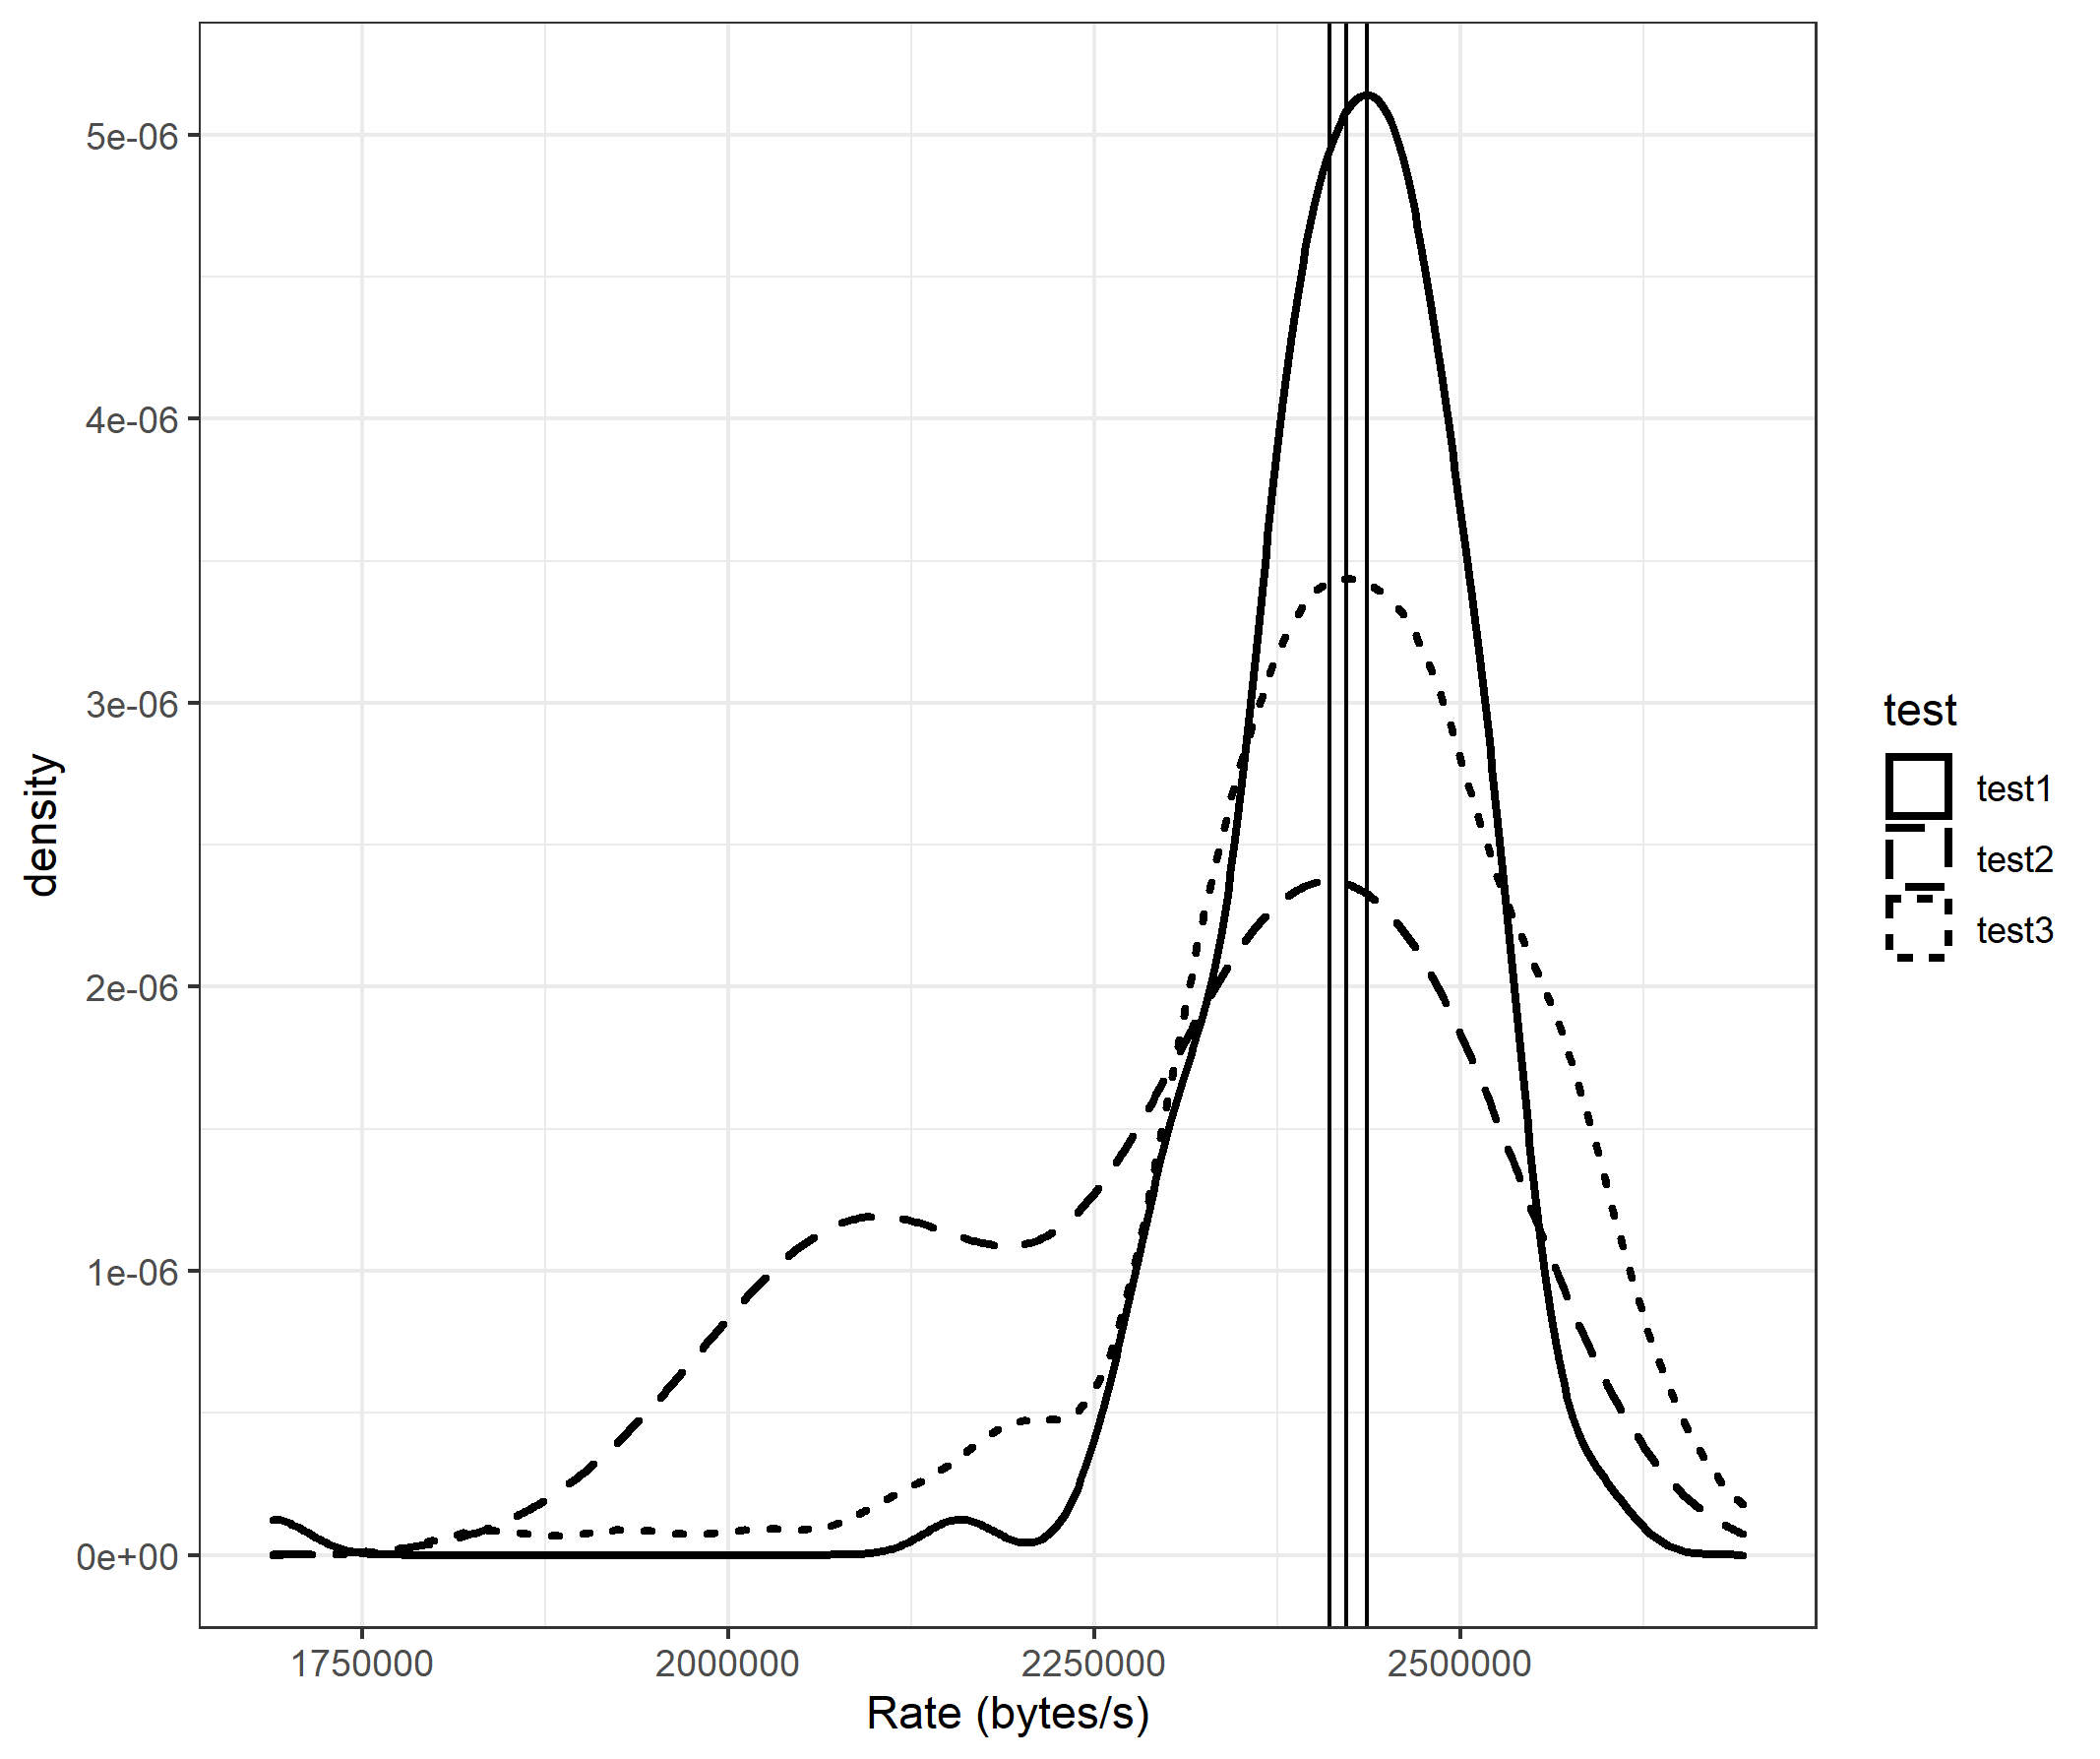
\includegraphics[width=0.7\textwidth]{images/consumer/density.png}
\caption{
    Density Plot for the consumer's measured throughput in the 3 testing
    conditions.
} 
\label{fig:consumer_capacity} 
\end{figure}

\subsubsection{Bin Capacity} \label{result:bin capacity}

Two measures are defined which are to be used in the sections to come. The
\lstinline[language=Python]{ALGORITHM_CAPACITY}, is the constant bin size that
will be used when running all the heuristic algorithms when solving the dynamic
BPP, whereas the \lstinline[language=Python]{CONSUMER_CAPACITY} is the
consumer's maximum capacity, which if exceeded, must trigger a new configuration
as for which partition should be assigned to which consumers.

The reason for having defined these two configuration parameters differently are
due to the problem's dynamic nature. Since the measured write speed for each
partition varies between each measurement, after executing the BPP algorithm for
a single measurement, it is common to have bin's filled close to their capacity,
which would lead to excessive rebalancing computations if the algorithm and
consumer capacity were defined using the same value. Defining the Consumer's
capacity to a value higher than the algorithm's perceived capacity, reduces the
number of rebalances triggered, at the cost of a reduced bin capacity. 

From graph \ref{fig:consumer_capacity}, the Consumer's capacity is set to $2
Mbytes$, whereas the Algorithm's capacity is defined as $1.5 Mbytes$.  These are
the values used for the remaining part of the work.  It is important to note
that these values are only valid when the consumers are deployed in the
environment where they were tested. Having executed the test in multiple
environments, it can be said that the consumer's maximum capacity does not
change between consumer instances as long as the environment is similar for all
consumers.

\section{Controller/Orchestrator} \label{component:controller}

The controller is the component of the system which is responsible for
orchestrating and managing the consumer group that is intended to consume the
data from the partitions of interest. 

The problem is modeled as a dynamic bin packing problem, where the size of each
item is equivalent to the write speed of each partition, and the size of the
container represents the maximum achievable speed of a consumer which has been
provided by the data presented in \ref{result:bin capacity}.

For clarity, for the following sections, consumer, container and bin will be
used interchangeably, representing a consumer instance described in
\ref{component:consumer}.

This problem is different to the usual bin packing problem due to the changing
write speed of each partition (the size of the items). This implies that a
viable solution in one iteration, might not be viable in a future iteration when
the sizes have changed.

At any given time, no consumer within the consumer group can have its capacity
exceeded by the cumulative write speed of the partitions assigned to it, and if
it is, then a rebalance has to be triggered. The same applies in case a
partition has not yet been assigned a consumer.

After the controller determines the state in which it wants its consumer group,
it then creates the consumers that don't yet exist, communicates the change in
assignment to each consumer in the group, followed by deleting the consumers
that are not required in the new computed group's state.

While rebalancing any partition, during the time the controller is informing the
current consumer to stop reading from it to inform the new consumer to start
doing so, the messages belonging to this partition are not being read. This is
the new cost that has to be taken into consideration when dealing with the
rebalancing procedure.

\subsection{System Design}

As has been described, there are three different components in the system that
work together to get the data from Kafka into bigquery. To do so, each component
has to be able to communicate with one another to inform any change in state.
For this reason, the following diagram describes how the pieces fit together,
and communicate with one another.

As shown in figure \ref{fig:system_architecture}, there are two main topics that
will be responsible for providing an asynchronous communication between the 3
different entities of the system. The \lstinline{monitor.writeSpeed} topic, is where
the monitor process sends the speed measurements for the controller to consult,
whereas the consumer.metadata topic is where the controller sends
messages to each consumer to inform the change in their state. Partition 0 of
this topic is reserved for the controller so the consumers always know how to
acknowledge their change in state.

When using a Kafka topic to communicate between the consumers and the controller
there are certain requirements that need to be complied with. 

The first, is that when the controller communicates with a consumer from the
consumer group, it has to be guaranteed that the message reaches the intended
consumer. 

Secondly, as will be common with this system, the controller will create and
delete a single consumer multiple times in its lifecycle. The message offset a
consumer starts on after restarting, has to be precisely the one where it left
off before being shut down by the controller. This can be done leveraging
kafka's \lstinline[language=Python]{group-id} property, defined in each consumer
client, and so the system just has to guarantee that the consumer gets the same
id as before.

Thirdly, each consumer only reads messages which are intended to it. This would
represent maximum efficiency in the information transmitted between both
controller and consumer, since no process is reading messages that have to be
ignored. To better understand this design requirement, the following scenario is
described: It might happen that a certain number of consumers satisfies the
controller's conditions, without any need to scale up or down the group. This
would imply that the control messages sent by the controller are only read by
the currently active consumers. When a new consumer is started by the
controller, if the messages are shared, then there is a big queue of messages
that have not yet been read by the new consumer since it was last up. For the
new consumer to be able to read new control messages sent by the controller, it
would first have to read all messages that were not intended to it prior to it
starting up.

Lastly, to guarantee temporal consistency in the control messages sent to a
single consumer, it is clear that a control message can only be sent to a single
partition, as kafka only guarantees message read order when the messages belong
to the same partition. Kafka already does this by allowing a message to have a
key attribute which is then hashed to determine the partition in which the
message is to be inserted. The issue with this approach is if the number of
partitions in the consumer.metadata topic increases, the key might not
send the messages to the same partition as before. As such, each consumer is
given an incremental id ($1, 2, ...$), which represents the partition where
change in state information has to be sent for the consumer to read (both
controller and consumer are aware of this id).

\subsection{State Machine}

The controller can be defined by a state machine, intended to continuously
manage a group of consumers and their assignments. A group's assignment
represents the same group's state.

The following diagram shows the high level architecture of the controller
process:

\begin{figure}[H] \centering
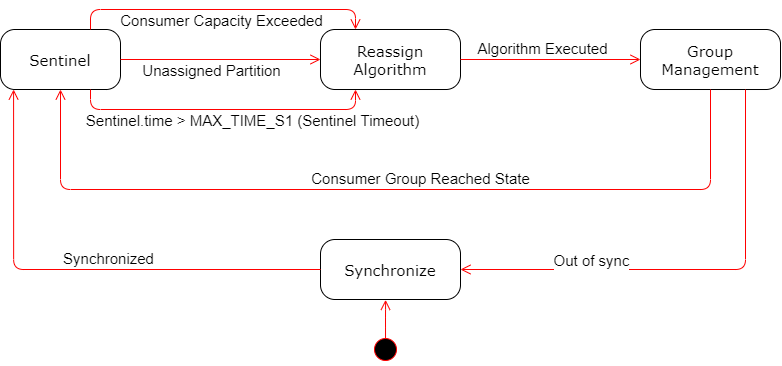
\includegraphics[width=\textwidth]{images/controller/state_machine.png}
\caption{Controller State Machine.} \label{fig:state_machine} \end{figure}

\subsection{State Sentinel}

This state is where the controller uses the information provided by the monitor
component (\ref{component:Monitor}), to determine whether it has to recompute
the consumer group's assignment. The first step the controller goes through in
this state is to read the last speed measurement the monitor component added to
the \lstinline{monitor.writeSpeed} topic.

The controller then updates each of the partition's speeds, which in turn
updates the cumulative speed of each consumer. As can be seen in figure
\ref{fig:state_machine}, there are three transitions that can lead to the
controller re-computing the current consumer group's assignment:
\begin{enumerate} \item \textbf{Consumer Capacity Exceeded} - This transition is
        triggered if the cumulative speed of all the partitions assigned to any
    consumer, exceeds the maximum consumer capacity measured in \ref{result:bin
capacity}.  \item \textbf{Unassigned Partition} - If there is any partition
    within the last speed measurement that is not currently assigned to a
        consumer, then this transition is triggered.  \item \textbf{Sentinel
            Timeout} - One of the controller's configurations, is a parameter
            \lstinline[language=Python]{MAX_S1_TIME} which indicates the maximum
            amount of time the controller can spend in the sentinel state
            without triggering a rebalance. This trigger is to have a condition
            that runs the algorithm to verify if downscaling is viable, as the
            other triggers are directed to upscaling conditions.
\end{enumerate}

\subsection{State Reassign Algorithm}

This state receives as input the current consumer group's assignment and the
remaining unassigned partitions, and produces as output a new consumer group
assignment, which is to be defined as the group's future state.

This state uses only approximation algorithms to determine the group's future
assignment. The algorithms implemented are the already existing Next Fit, First
Fit, Worst Fit, Best Fit, and each of the previous algorithms' decreasing
versions, and modified versions of the Best and Worst Fit algorithms. 

In the implementation of the existing approximation algorithms, another step was
included during the creation of the bins which does not affect the outcome in
terms of number of consumers. If the consumer that is currently assigned to the
partition has not yet been created in the future assignment, this is the bin
that is created, otherwise, the lowest index bin that does not yet exist is the
one created.
 
\begin{figure}[H] \centering
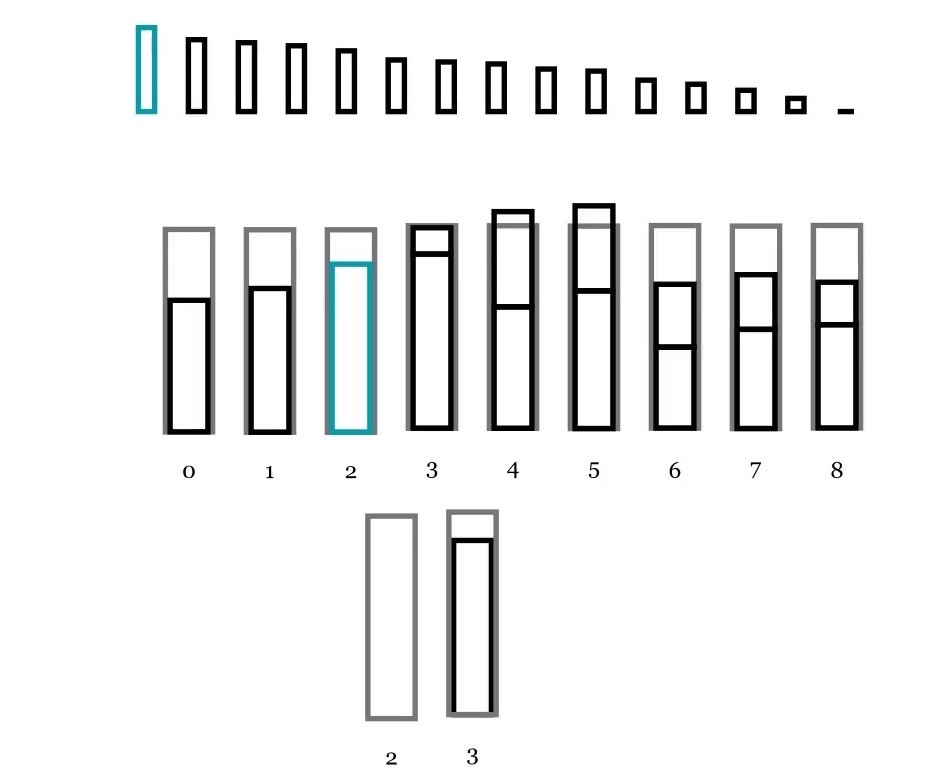
\includegraphics[width=0.6\textwidth]{images/controller/ApproximationAlgorithm_NewBin.png}
\caption{New bin creation procedure when performing an approximation algorithm.}
\label{fig:approximation_bin_creation} \end{figure}

Figure \ref{fig:approximation_bin_creation} illustrates this process, wherein
the first row of consumer's (grey containers) represents the current consumer
group's state, and the second the new consumer group assignment that is being
computed by the controller. Partitions are represented in red and white, red
being the partition currently being analyzed by the controller. In this example,
the red partition currently finds itself in the consumer 2. When analysing the
partition, the controller verifies if the partition fits in any of the existing
partitions. Since it does not fit, and another consumer has to be created for
this partition, the new consumer is the same as the one it is currently
assigned, therefore occurring no rebalance for this partition.

This is not presented as a modification to these algorithms as their
functionality does not change with this approach to for a bin's creation, as it
simply adapts the algorithms to the rebalancing problem at hand, improving it as
compared to always creating the lowest index bin, as that would imply
rebalancing partitions more often.

\subsubsection{Modified Any Fit Algorithms}
\label{subsub:modified_any_fit}

The motivation to modifying the existing Any Fit algorithms, is that the item
reassignment is not the problem they are trying to solve, they simply aim to
reduce the amount of active bins for a certain list of items. 

Within this problem's context, rebalancing inevitably implies having the
consumer group to stop consuming from a partition, while the controller is
reassigning the partition from one consumer to another (as there cannot be a
concurrent read from the same partition).

A new measure is presented to compute the the total rebalance cost (Rscore), of
a new group's configuration. This metric represents the rate at which
information is accumulating for each second that passes, given in consumer
iterations per second.

\begin{table}[H] \centering \caption{Data to compute the Rscore for an
    iteration.} \begin{tabular}{ |c|l| } \hline \textbf{Symbol} &
        \textbf{Description} \\ \hline $P_i$ & set of partitions that were
        rebalanced in iteration $i$ \\ $s(p)$ & outputs the write speed of
        partition $p$ \\ $R_i$  & Computed total Rscore for iteration $i$ \\ $C$
    &  Constant that represents the maximum consumer capacity from
    \ref{result:bin capacity}\\ \hline \end{tabular} \end{table}

The following equation then presents the cost of rebalancing for a single
    iteration $i$.

\begin{equation} R_i = \frac{1}{C}\sum_{p \in P_i} s(p) \end{equation}

Since the controller has access to the speed measurements of all partitions and
    it does not require to read and assign each partition in any particular
    order, this bin packing problem can be categorized as offline.

Different from the previous decreasing versions of the Any Fit algorithms which
    have already been described in \ref{sub:Approximation Algorithms and
    Heuristics}, this algorithm will not sort the partitions, but in turn the
    consumers (bins).

There will be 2 main approaches to sorting the consumers: \begin{itemize} \item
        Sorting each consumer based on their current cumulative speed
    (cumulative sort); \item Sorting each consumer based on the partition
        assigned to it that has the biggest measured write speed (max partition
        sort).  \end{itemize}

After sorting the current consumer group using one of the above strategies, the
    procedure is as follows:

\IncMargin{1em} \begin{algorithm}[h]
    \SetKwData{Left}{left}\SetKwData{This}{this}\SetKwData{Up}{up}
    \SetKwFunction{Union}{Union}\SetKwFunction{FindCompress}{FindCompress}
    \SetKwInOut{Input}{input}\SetKwInOut{Output}{output} \Input{current consumer
    group C and set of unassigned partitions U} \Output{consumer group N which
    is the next state for the consumer group} \BlankLine N $\leftarrow$ new
    ConsumerList(assign\_strategy=("BF" | "WF"))\; sorted\_group $\leftarrow$
    sort(C, sort\_strategy=("cumulative" | "max partition"))\; \For{consumer
    $\in$ sorted\_group}{ Set<Partition> partitions $\gets$
    consumer.assignedPartitions()\; List<Partition> sorted\_partitions
    $\leftarrow$ sort(partitions, reverse=True)\; \For{i $\leftarrow$
    length(sorted\_partitions)-1 \KwTo 0}{ partition $\leftarrow$
    sorted\_partitions[i]\; result $\leftarrow$ assignExisting(N, partition)\;
    \If{result $==$ False}{ break\; } remove(sorted\_partitions, partition)\; }
    \If{sorted\_partitions.length() == 0}{ continue\; } createConsumer(N,
    consumer)\; \For{partition $\in$ sorted\_partitions}{ result $\leftarrow$
    assignCurrent(N, partition, consumer)\; \If{result $==$ False}{ break\; }
    remove(sorted\_partitions, partition)\; } extend(U, sorted\_partitions)\; }
    sorted\_unassigned $\leftarrow$ sort(U, reverse=True)\; \For{partition $\in$
    sorted\_unassigned}{ assign(N, partition)\; } \KwRet{N} \caption{Modified
Any Fit Pseudo Code}\label{algo:MBPP} \end{algorithm}\DecMargin{1em}


For each consumer in the sorted consumer group, the partitions assigned to the
    consumer are sorted based on their write speed. From smallest to biggest,
    each partition is inserted into one of the bins that have already been
    created in the future assignment, based on one of the any fit strategies,
    which in the tested implementation, can either be with a Best or Worst Fit
    strategy. If the insert is successful, then the partition is removed from
    the sorted list of partitions, otherwise, if there is no existing bin that
    can hold the partition, then the current consumer assigned to it is created. 

The remaining partitions in the sorted list are now inserted into the newly
created bin, from biggest to smallest, and removed from the sorted list if
successful. If a partition does not fit into the newly created consumer, then
the remaining partitions in the list of sorted partitions are added to the set
of unassigned partitions.

After performing the same procedure over all consumers, there is now a set of
partitions which have not been assigned to any of the consumers in the future
assignment. These partitions are first sorted in decreasing order (based on
their measured write speed), and each partition is assigned using their
respective any fit strategy.

\begin{table}[H] \centering \caption{Modified implementations of the any fit
    algorithms.} \begin{tabular}{ |c|c|c| } \hline \textbf{Algorithm} &
        \textbf{Assign Strategy} & \textbf{Consumer Sorting Strategy} \\ \hline
        Modified Worst Fit & Worst Fit & cumulative write speed \\ Modified Best
        Fit & Best Fit & cumulative write speed \\ Modified Worst Fit Partition
        & Worst Fit & biggest partition write speed \\ Modified Best Fit
        Partition &  Best Fit & biggest partition write speed \\ \hline
    \end{tabular} \end{table}

\subsubsection{Testing} \label{c3subsub:testing}

To evaluate the performance of each of these algorithms, two metrics were used:
    The relative difference in the number of consumers of each algorithm to the
    approximation algorithm that presented the least amount of consumers; The
    Rscore of the algorithm's new configuration.

\begin{table}[H] \centering \caption{Data to create the testing environment for
    the approximation algorithms.} \label{table:testing_data} \begin{tabular}{
            |c|l| } \hline \textbf{Symbol} & \textbf{Description} \\ \hline $P$
        & Set of partitions assigned to the consumer group. \\ $s_p^i$ &
    Provides the speed for partition $p$ in iteration $i$ \\ $\phi(\delta)$ &
    Uniform random function that selects a value between $[-\delta, \delta]$\\
    \hline \end{tabular} \end{table}

Given the data provided by \ref{table:testing_data}, the testing sequences for
the algorithms was obtained as follows: \begin{enumerate} \item 200 different
            partitions are created and given an initial speed. Four different
            initial conditions for all partition were tested: Starting at $0\%$
            of the \lstinline[language=Python]{ALGORITHM_CAPACITY}; Starting at
            $50\%$ of the \lstinline[language=Python]{ALGORITHM_CAPACITY};
            Starting at $100\%$ of the
            \lstinline[language=Python]{ALGORITHM_CAPACITY}; Assigning each
            partition a uniform random value between $[0, 100]\%$ of the
            \lstinline[language=Python]{ALGORITHM_CAPACITY}.
    
    \item Given the initial conditions, a new measurement is created, where the
        speed in the next measurement is calculated using: \begin{equation}
        s_p^{i+1} = s_p^i + \phi(\delta) \times algorithm\_capacity, \quad
        \forall p \in P, \end{equation} having $\phi(\delta)$ be evaluated every
        new computation.
    
    \item The previous step is repeated for the next measurements until there
are 500 measurements in a single sequence.  \end{enumerate}

Using this procedure, six different sequences of measurements were created, each
    differing in the $\delta$ used to vary the speed. As such, for each initial
    condition, there is a sequence where $\delta$ is set to $0, 5, 10, 15, 20,
    25$. In other words, there are $6 (deltas) \times 4 (starting\; conditions)$
    different sequences, each representing a measurement instance provided by
    the monitor process. After reading a single measurement from a sequence, the
    controller runs the implemented algorithms to find the group's configuration
    in all scenarios.

\begin{figure}[H] \centering
    \includegraphics[width=0.8\textwidth]{images/controller/Relative Number of
    Consumers.png} \caption{Average Relative Deviation from the configuration
    that provides the minimum number of consumers, with a random initial speed
    for each partition.} \label{fig:relative_nconsumers} \end{figure}

To better illustrate the performance of the algorithms for each measurement
    sequence, the metrics are statistically summarized using the average. The x
    axes refers to the 6 different measurement sequences for a given starting
    condition, and the value is the $\delta$ defined for that measurement. As
    for the y axes in \ref{fig:relative_nconsumers}, it indicates the
    algorithm's average relative deviation from the configuration that provides
    the minimum number of consumers.

In \ref{fig:relative_nconsumers}, each partition starts with a random speed
    between $[0,100]\%$ of \lstinline[language=Python]{ALGORITHM_CAPACITY}. The
    worst performing algorithm is the next fit followed by its decreasing
    version, since every time a partition is to be assigned, the algorithm only
    verifies if it fits in the last created bin, as opposed to considering all
    the already existing bins. The remaining any fit decreasing algorithms, are
    the ones that perform the best, with the best fit decreasing consistently
    presenting the best results. 

\begin{figure}[H] \centering
    \includegraphics[width=0.7\textwidth]{images/controller/Relative Number of
    Consumer Modified.png} \caption{Average Relative Deviation from the
    configuration that provides the minimum number of consumers, with a random
    initial speed for each partition. (Filtered to present the modified
    algorithms and BFD)} \label{fig:relative_nconsumers_modified} \end{figure}

As for the modified versions of these algorithms, due to its sorting strategy,
MBFP shows the best results. It is also worth noting that for smaller
variabilities, the modified algorithms behave similarly to the online versions
of their any fit strategy, but, the higher the delta, the bigger the
variability, which also leads to more rebalancing, having the modified
algorithms behave more like the decreasing versions of their fit strategy.

\begin{figure}[H] 
    \centering
    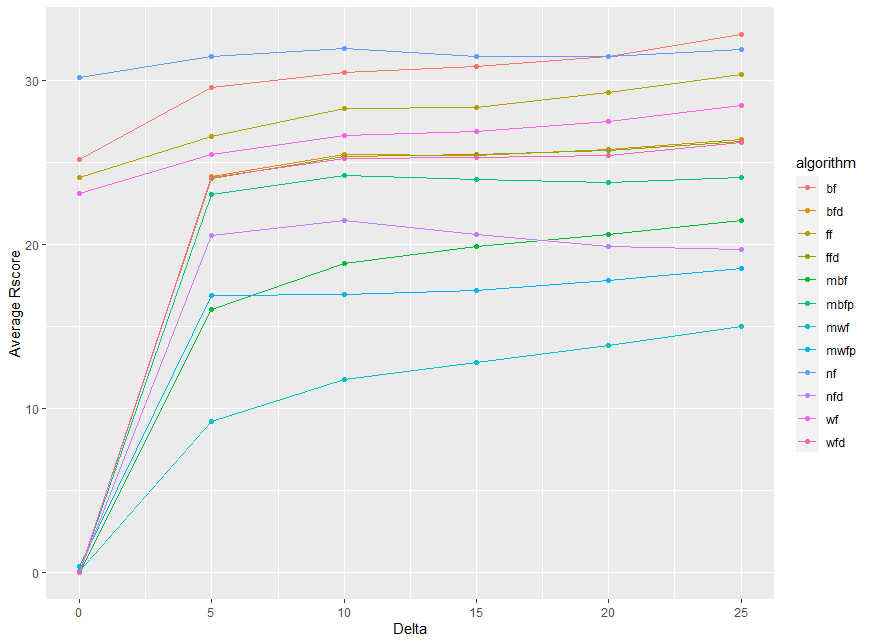
\includegraphics[width=0.7\textwidth]{images/controller/Rscore.png}
    \caption{
        Impact on Rscore for different Deltas (random initial partition speed).
    } 
    \label{fig:rscore} 
\end{figure}

For the same starting conditions, \ref{fig:rscore} presents the average Rscore
of each algorithm for all six measurement sequences.

As can be seen in \ref{fig:rscore}, the modified algorithms present the best
Rscore for each measurement along with next fit decreasing. The reason why the
NFD presents such a result, is due to the increased amount of consumers it
creates to assign new partitions, which at the moment of creation, will always
be the same consumer as the one assigned to the partition being analyzed, as
long as it has not yet been created (\ref{fig:approximation_bin_creation}).

For a similar reason, the modified algorithms that perform the best with regards
to the Rscore, are also the ones that perform worst (compared to the remaining
modified algorithms) when evaluating the relative number of consumers.

The remaining tests performed are presented in the appendix, and it can be
concluded, that the initial conditions do not significantly affect the relative
performance of the algorithms (\ref{}).

To select the algorithm to use within the controller, there is a trade-off
between the aforementioned testing metrics. On account of the added re-balance
concern within the modified algorithms, these present an improvement with
regards to the Rscore compared to the approximation algorithms presented in the
literature.

\begin{figure}[H] \centering
\includegraphics[width=\textwidth]{images/controller/Facet Wrap Pareto
Front.png} \caption{Pareto Front for each delta value used in the measurement
sequences.} \label{fig:pareto_front} \end{figure}

The pareto front is a way of evaluating the set of solutions that are most
efficient, provided there are trade-offs within a multi-optimization problem.

Excluding MWFP, the modified algorithms are consistently a part of the pareto
front \ref{fig:pareto_front}, which implies these are a competitive option as to
which algorithm to pick for the reassign algorithm to be executed in the
controller. The algorithm that shows the best Rscore for the different
variabilities is the MWF, whereas the modified algorithm that performs the best
relative to the number of consumers used in each configuration is the MBFP.

\subsection{State Group Management}

This state is where the controller informs each consumer of their change in
state. Since there cannot be any concurrent read of a partition by two consumers
of the same consumer group, when rebalancing a partition, the controller first
has to inform the consumer currently assigned to the partition to stop consuming
from it, and only after the consumer acknowledges having acted to the request,
can it inform the new consumer of its new assignment.

This state not only handles this message exchange but it also creates and
deletes consumer resources from the Kubernetes cluster. 

\subsubsection{Difference between current and future state}

The current consumer group's state is represented by a list of consumers, each
having their own assignment. The new computed group's state is defined as the
next state, and is also a list of consumer's each having an assignment, but
representing the desired state the controller will communicate to each consumer.

Similar to computing the difference between two sets, when computing the
difference between 2 consumer lists the procedure involves iterating over each
consumer (in both states), and calculate the difference between the two consumer
assignments (set of assigned partitions). There are three scenarios that result
in different actions the controller has to perform, for a given position $i$ of
each consumer list: \begin{itemize} \item next state has a consumer at $i$ but
            the current state does not - This means that the consumer has to be
            created by the controller, and the partitions assigned to the
            consumer in position $i$ of the next state, have to be associated
            with a StartConsumingCommand for this same consumer.  \item next
                state does not have a consumer at $i$ but the current assignment
                does - The partitions associated with the consumer at position
                $i$ of the current state have to be associated with a
                StopConsumingCommand directed to this consumer, and the consumer
                has to be added to the list of consumers to remove.  \item both
                    next state and current state have a consumer at position $i$
                    - This means that no creation or deletion operation has to
                    be performed for this bin, and the operations to perform in
                    this case are only communicating to the already existing
                    consumer the difference in its assignment. 
    
    The same consumer has two different sets of partitions assigned to it
        represented in the two different group states.
        \lstinline[language=Python]{next_assignment} will denote the set of
        partitions attributed to the consumer's state in the next group's
        context, and \lstinline[language=Python]{current_assignment} is defined
        as the consumer's set of partitions in its current state.
    
    \begin{lstlisting}[language=Python] partitions_stop = current_assignment -
    next_assignment partitions_start = next_assignment - current_assignment
    \end{lstlisting} the resulting set of partitions within
        \lstinline[language=Python]{partitions_stop} have to included in a
        StopConsumingCommand, whereas the partitions in
        \lstinline[language=Python]{partitions_start} in a
        StartConsumingCommand, both message types directed to consumer $i$.
\end{itemize}

\subsubsection{Managing the Consumer Group in the Kubernetes Cluster}

Each active consumer in the current group's state, represents a deployment with
a single replica (pod). The reason why this is the case is that each consumer
requires a volume to persist its data, which implies having a different volume
for each pod. This is also possible using stateful sets, but the constraint of a
stateful set is that when removing a replica of the set, it only allows to
remove the last added replica, and in this context, a more granular approach is
required when removing an active consumer, as it does not necessarily have to be
the highest indexed consumer.

Each consumer is given an individual id through its deployment's
\lstinline[language=Python]{metadata.name} property, a value that can be
obtained within the pod using the downwardAPI, that provides a pod with its
context. This individual id assigned to the deployment's name, is the one used
to inform the pod of its metadata partition to consume from.

To allow the controller to create, list and delete the resources within the
cluster, a Kubernetes service account is used to authenticate the controller,
which is then given permissions for the aforementioned operations through a
Kubernetes Role. In this scenario, the controller's service account is linked
with a Role object that has permissions to create, list and delete, deployment
and persistent volume claim resources.

Since all consumers have to be able to persist data, each consumer has to be
mapped to a persistent volume using a persistent volume claim. If it is the
first time a consumer with a given id is being spawned, the controller has to
dynamically create and map a persistent volume claim to the consumer's
deployment.

To simplify the process, two template yaml files (\ref{appendix:template-pvc},
\ref{appendix:template-consumer}) are used, one for creating persistent volume
claims (PVC), and another used to create deployments. The controller is only
responsible for changing the template PVC id when creating it. When the
controller has to create the deployment, it has to reference the created PVC in
the template deployment, and change the deployment's id to the incremental id
attributed by the controller.

As an example, if the controller has to create a consumer whose id is $5$, it
would go through the following steps: \begin{enumerate} \item If the PVC with
            name \lstinline[language=Python]{de-consumer-5-volume} does not yet
            exist, change the PVC metadata.name parameter to
            \lstinline[language=Python]{de-consumer-5-volume}, and send the
            create request with the body containing the modified yaml file;
        \item Change the template deployment's metadata.name parameter to
            \lstinline[language=Python]{de-consumer-5}, and add a reference to
            the PVC created in the previous step.  \end{enumerate}

\subsubsection{Communication between controller and Consumer Group}
\label{sub:controller_communication_cosumer}

Using the computed difference between the next and current group's state, each
consumer has a set of start and stop messages that have to be sent by the
controller, for the group to reach the intended state.

Each partition can have associated to it, at most two actions, which correspond
to a start and/or a stop command. 

Firstly, the controller prepares a batch of StartConsumingCommand messages, each
directed to a single consumer. For each partition in the set of unassigned
partitions, the partition id is added to the StartConsumingCommand message that
is intended to the consumer that was assigned the partition.

Another batch of StopConsumingCommand messages is prepared, and for each
partition that has to be either rebalanced or removed, that partition's id is
added to the message which is intended to the consumer that is currently
assigned to that partition. 

Each message the controller sends out to a consumer, has to be acknowledged by
the consumer with a corresponding event which can be one of two types,
StartConsumingEvent, StopConsumingEvent. Each of these messages contain a set of
partitions from which a consumer acted upon. For each partition contained within
one of the events, the controller removes its corresponding actions from the set
of actions that have to be deployed by the controller. 

If the received event is of type StopConsumingEvent, a new batch of
StartConsumingCommand records are prepared for the consumers that have to start
consuming from the partitions that are being rebalanced. This means that for
each partition referred in the StopConsumingEvent, if it has a corresponding
start action, the partition is added to the StartConsumingCommand directed to
the new consumer. 

When the controller sends a message to a consumer, it sends it to the same
partition as the consumer's id in the consumer.metadata topic. As for
the consumer, to communicate the event of having reacted to one of the
controller's commands, the record has to be sent to the partition with id $0$ of
the same topic, as depicted in the diagram (\ref{fig:system_architecture}).

This process terminates when there are no more actions to perform over any
partition, since the controller removes a start or stop action from a partition
as soon as it receives the acknowledgement by the consumer that it has performed
the corresponding command.

\subsection{Synchronize}

The controller enters this state if the state it holds of the consumer group,
which is the state it has for each active consumer, is not synchronized with the
state in each consumer. 

This state was then created to mitigate this problem, following a procedure
which has the controller querying the kubernetes cluster to verify which are its
active consumers. Given this, the controller then queries each consumer through
their respective partitions for their current state, and only after all active
consumers have responded does the controller proceed to its normal behaviour
triggering the transition to the Sentinel state.

While testing the controller, this state would most commonly be triggered after
the controller would unexpectedly fail and then restart.
